% All numbers come from ../data_v3 (generated by ../src_v3).
\documentclass[11pt]{article}
\usepackage[utf8]{inputenc}
\usepackage[T1]{fontenc}
\usepackage{amsmath,amssymb}
\IfFileExists{mathdesign.sty}{\usepackage[bitstream-charter]{mathdesign}}{\usepackage{lmodern}}
\usepackage{booktabs}
\usepackage{graphicx}
\usepackage[section]{placeins}
\usepackage[margin=1in]{geometry}
\usepackage{xcolor}
\usepackage[colorlinks,linkcolor={red!50!black},citecolor={blue!50!black},urlcolor={blue!80!black}]{hyperref}
\usepackage{lineno}
\usepackage[english]{babel}
\urlstyle{same}
\providecommand{\doi}[1]{\href{https://doi.org/#1}{doi:\,#1}}
\DeclareSymbolFont{usualmathcal}{OMS}{cmsy}{m}{n}
\DeclareSymbolFontAlphabet{\mathcal}{usualmathcal}
\graphicspath{{../figures_v3/}}
\newcommand{\ohmcm}{\ensuremath{\Omega\cdot\mathrm{cm}}}
\newcommand{\ohmum}{\ensuremath{\Omega\cdot\mu\mathrm{m}}}
\sloppy

\title{Gate-Controlled Hole Injection at Top and Edge Contacts to Few-Layer InSe:\\ An Anisotropic, Electro-Thermal TCAD Study Verified Analytically and Benchmarked on a Known Contact}
\author{Harsha Adhikary\thanks{Corresponding author. Email: \href{mailto:harshaa@iisc.ac.in}{harshaa@iisc.ac.in}} \\[4pt]
\small Department of Physics, Indian Institute of Science (IISc), Bengaluru, India}
\date{}

\begin{document}
\maketitle

\begin{abstract}
\noindent
We model hole injection into back-gated few-layer $\gamma$-InSe through top and edge metal contacts with an open-source DEVSIM model that couples Fermi--Dirac drift-diffusion with anisotropic mobility, flux-balanced thermionic emission across the van der Waals (vdW) gap, nonlocal Tsu--Esaki tunnelling, and an anisotropic lattice heat equation with Joule, Peltier and tunnelling heat. Nine tests verify it against closed-form results and conservation laws. With one parameter fitted to ultra-high-vacuum Au/MoS$_2$ contacts it predicts the measured transfer length (34 against 35--40~nm). Reproducing the InSe contact measurements of Chen \textit{et al.}, it recovers the reported pinning factors and, for an assumed mobility of 100--200~cm$^2$/Vs, the 3--6$\times$ on-current gain of their oxide interlayer. With the measured direct-contact pinning ($S=0.05$) every metal gives a hole barrier of 1.05--1.12~eV; holes are then injected almost entirely by gate-induced tunnelling, and the metal hardly matters (2.4$\times$ from Ti to Pt). Depinning is the first lever: with the oxide interlayer ($S=0.5$) Pt reaches 0.52~eV and a contact-limited on-state resistance up to 700$\times$ lower. Geometry is the second: in the gated on state edge contacts beat 50-nm top contacts by a margin growing from 14$\times$ at 0.2~eV to 150$\times$ at 1.0~eV, because they tunnel in-plane, avoiding the vdW gap and slow out-of-plane transport. This advantage survived independently varied pinning in 96\% of Monte Carlo samples; without a gate it is lost if edge contacts are more strongly pinned. Self-heating matters only after depinning. A compact model reproduces top-contact resistance to 11\% (median).
\end{abstract}

\noindent\textbf{Keywords:} indium selenide; Schottky-barrier FET; contact resistance; tunnelling; electro-thermal simulation; van der Waals contacts

\linenumbers

\section{Introduction}
InSe combines high electron mobility \cite{refband}, ballistic short-channel transistors \cite{refjiang} and wafer-scale growth \cite{refqin}, but complementary logic also needs efficient hole injection, which has received far less attention \cite{refsong}. Metal contacts to 2D semiconductors are governed by the Schottky barrier and Fermi-level pinning, by the vdW tunnel gap of top-deposited metals, and by how current spreads from the contact into the channel \cite{refallain,refkang}. Edge contacts remove the vdW gap and inject in-plane \cite{refwang,refguim}. Real devices are gated, and the gate can thin the Schottky barrier until tunnelling dominates injection, as in Schottky-barrier FETs. Layered crystals are also strongly anisotropic. Carrier mobility across InSe layers is typically one to three orders of magnitude lower than along them \cite{refsangwan}, and the through-plane thermal conductivity is about eleven times lower \cite{refrai}.

This paper asks which contact geometry gives the lowest resistance for hole injection into a few-layer InSe p-FET, and why. It also asks how robust that answer is to the interface parameters, and what the measured Fermi-level pinning of InSe contacts \cite{refchen,refguo} implies for p-type operation. Edge and top contacts have been compared for MoS$_2$ with ab initio quantum transport \cite{refszabo,refparto} and with semiclassical injection models \cite{refarutchelvan}, and the vdW gap is known to penalise top contacts \cite{refkang}. These studies address electron injection into MoS$_2$. Hole injection into a strongly anisotropic layered semiconductor, through a gate-controlled tunnelling path and with self-heating, has not been treated. We use a drift-diffusion model with a flux-balanced contact condition, non-equilibrium Poisson coupling, Fermi--Dirac statistics, a gate, nonlocal tunnelling, transport and thermal anisotropy and a complete heat source, verify each ingredient, and benchmark the numerics on Au/MoS$_2$. The contributions are:
\begin{itemize}
\item the finding that the edge-contact advantage for holes \emph{grows} with the barrier under gated tunnelling (from 4$\times$ to 150$\times$) and survives unequal pinning in the on state;
\item the consequence of the measured pinning: direct metal/InSe contacts have a hole barrier of about 1.1~eV regardless of the metal, so depinning must precede geometry;
\item a reproduction of the InSe contact measurements of Ref.~\cite{refchen}, which recovers the pinning factors and the on-current gain of the oxide interlayer once the unreported mobility is taken into account;
\item open code and data that regenerate every quoted number.
\end{itemize}

\section{Model}
\label{sec:model}
\subsection{Device and band structure}
The two geometries are sketched in Fig.~\ref{fig:schem}. The device is an $N$-layer InSe film (0.83~nm per layer; $N=6$, $t=5$~nm by default) on 10~nm SiO$_2$ with a back gate (flat band at $V_G=0$), with a 50-nm channel. Top contacts of length $L_c$ cover the upper surface, and edge contacts cover the film's end faces. The band gap follows a fit to photoluminescence data \cite{refmudd,refmudd2013}, $E_g(N)=1.26+2.78N^{-1.70}$~eV, which gives 1.69~eV at 3 layers, 1.39~eV at 6 layers and 1.30~eV at 12 layers. 32\% of the confinement shift is assigned to the valence band, roughly $m_e/(m_e+m_h)$. The 6-layer film therefore has $E_V=5.00$~eV below vacuum (Sec.~\ref{sec:thick}). All parameters and their provenance are listed in Table~\ref{tab:params}. Unless stated otherwise, results use this \emph{reference alignment} with $S=1$, which isolates the effects of geometry, transport and tunnelling at a given barrier. Section~\ref{sec:measured}, and the results labelled `measured alignment' in Secs.~\ref{sec:thick}, \ref{sec:heat} and~\ref{sec:uq}, instead use the measured electron affinity $\chi=4.6$~eV of bulk InSe \cite{refchen}, which places $E_V$ of the 6-layer film at 5.90~eV, together with the measured and calculated pinning of InSe contacts. Calculated ionisation energies are lower, about 5.2~eV \cite{refguo}, so the absolute alignment is uncertain by several tenths of an eV; results are therefore also given versus the hole barrier $\phi_{Bp}$, which is the quantity that matters.

\begin{figure}[!htbp]
\centering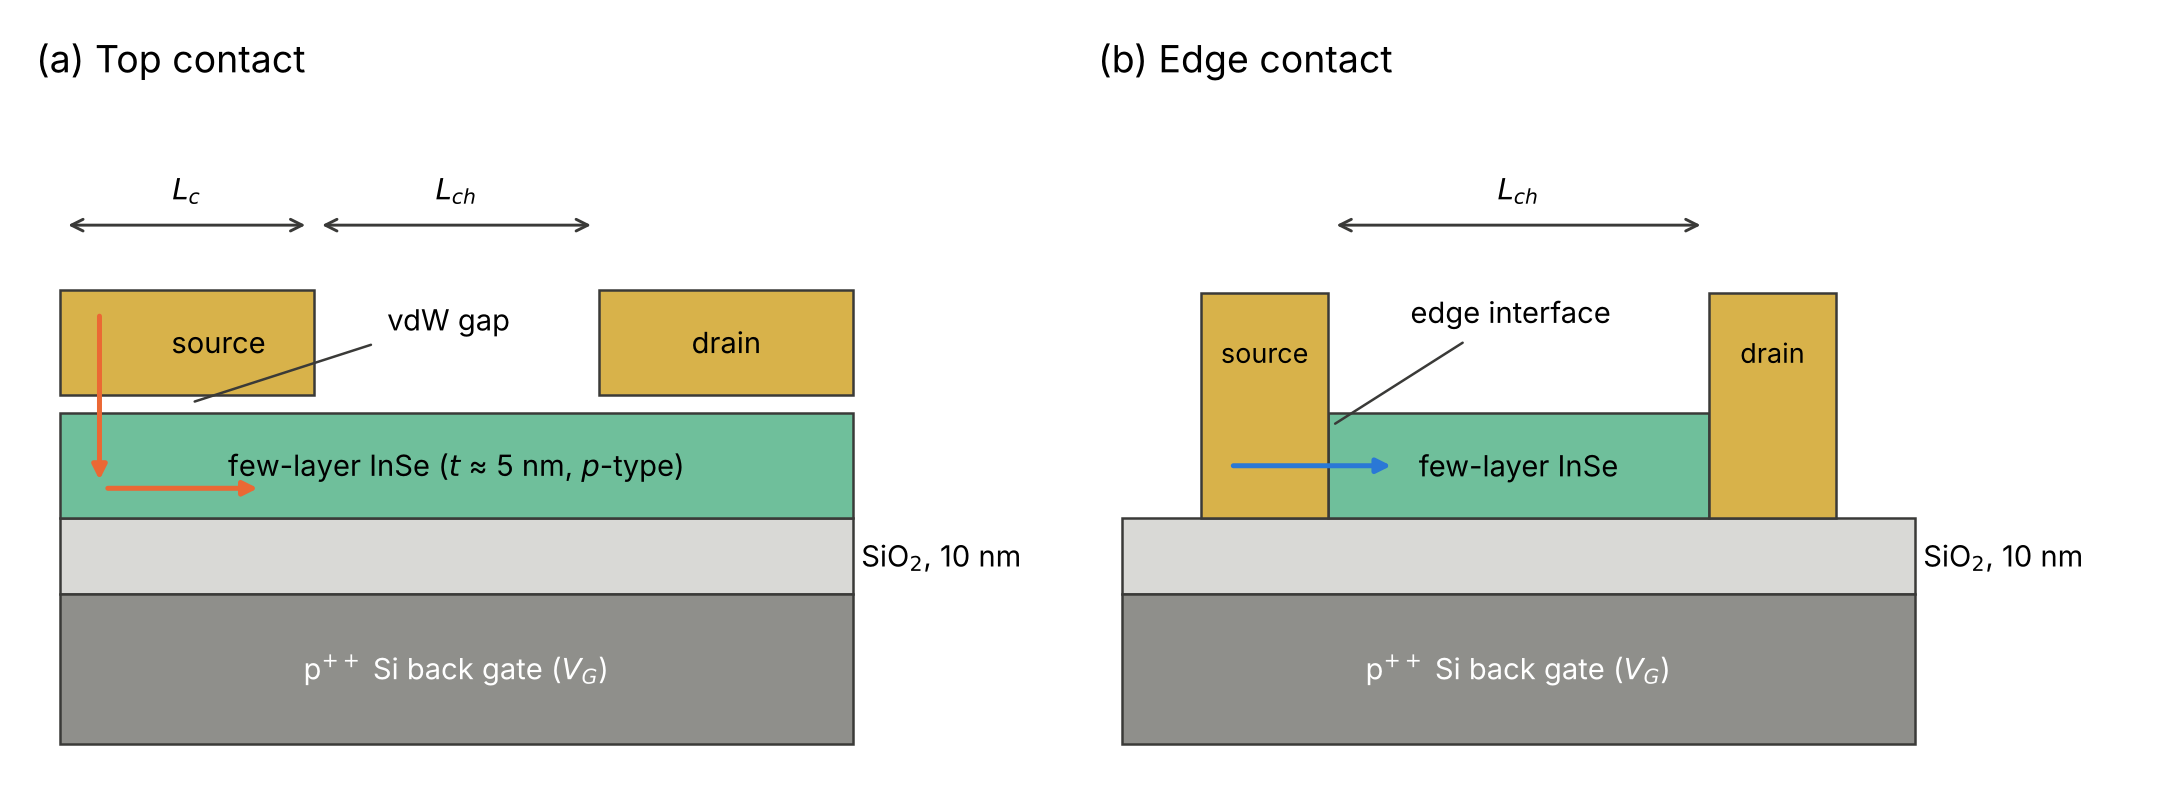
\includegraphics[width=0.96\textwidth]{fig0_device_schematic.png}
\caption{Simulated geometries (not to scale). (a) Top contacts of length $L_c$ separated from the film by a van der Waals gap; holes cross the gap and then flow laterally. (b) Edge contacts abutting the end faces of the film. Both devices sit on 10~nm SiO$_2$ with a back gate.}
\label{fig:schem}
\end{figure}

\begin{table}[!htbp]
\centering
\caption{Parameters (6-layer InSe unless stated). M: measured; L: literature calculation or compilation; R: representative value within a measured range; A: assumed. The last column gives the effect of a larger value on the on-state resistance (or on $\Delta T_{\max}$), from the Monte Carlo analysis (Sec.~\ref{sec:uq}) and the sensitivity runs, and the expected change for thinner films where it is known.}
\label{tab:params}\footnotesize
\setlength{\tabcolsep}{3pt}
\begin{tabular}{@{}p{0.17\textwidth}p{0.25\textwidth}p{0.21\textwidth}p{0.33\textwidth}@{}}
\toprule
Parameter & Value & Source / type & Effect of a larger value; thickness trend \\
\midrule
$E_g(N)$, $E_V(N)$ & $1.26+2.78N^{-1.7}$ eV; 1.39, 5.00 eV at $N=6$ & fit to PL \cite{refmudd,refmudd2013} (M); 32\% VB share (A) & Deeper $E_V$ raises $\phi_{Bp}$ and $R$ exponentially. Thinner films: larger gap, higher $R$ (Sec.~\ref{sec:thick}); VB share 0.2--0.5 moves the top-contact optimum by one layer \\
$m_e$, $m_h$ (DOS and tunnelling) & 0.07, 0.17 $m_0$ & L \cite{refmag} & Heavier $m_h$ suppresses tunnelling and raises the gated $R$ (second-largest index). Few-layer value uncertain; direction unknown \\
$\varepsilon_r$ & 6.4 & L & Raises the gated $R$ moderately ($\rho\approx0.2$--0.3). Weaker screening in few layers would lower $R$ \\
$\mu_{n,\parallel}$, $\mu_{p,\parallel}$ & 1000, 50 cm$^2$/Vs & M \cite{refband}; A & Lowers only the channel part; contact-limited on state insensitive (index at noise floor). Thinner films: lower $\mu$, higher $R_{\rm ch}$ \\
$\mu_\perp/\mu_\parallel$ & 0.01 (range 0.002--1) & M (electrons; 0.002 in vertical FETs \cite{refsangwan}, $\sim$0.01 bulk) & Smaller ratio raises top-contact $R$ (2$\times$ from 1 to 0.002, ungated); edge unaffected \\
$\mu(T)$ & $\propto T^{-1.5}$ & A & Stronger decay raises $R$ of self-heated devices only \\
$\kappa_\parallel$, $\kappa_\perp$ & 8.5, 0.76 W/mK & M, time-domain thermoreflectance \cite{refrai} & Lower $\kappa$ raises $\Delta T_{\max}$ (measured vs isotropic $\kappa_\perp$: +8--17\%). Few-layer $\kappa$ likely below bulk: higher $\Delta T$ \\
$c_V$ & 1.43 J/cm$^3$K & Dulong--Petit (L) & Scales only the thermal time constant \\
$N_A$ & $10^{16}$ cm$^{-3}$ & A & Weak (index at noise floor) \\
$S_{\rm top}$, $S_{\rm edge}$, $\Phi_{\rm CNL}$ & 1, 1, 4.35 eV (reference); 0.05 and 0.5 measured, 0.18 calculated (Sec.~\ref{sec:measured}) & A (varied); M \cite{refchen}; L \cite{refguo} & Dominant: the pinning level and $S$ set $\phi_{Bp}$ (largest indices); for Pt a larger $S$ lowers $R$. $S_{\rm edge}>S_{\rm top}$ reverses the ungated ranking only \\
vdW gap $d$, $\Phi_{\rm vdW}$ & 0.30 nm, 2.0 eV ($\mathcal{T}_{\rm vdW}=0.013$) & A (varied) & Raise top-contact $R$ only ($\rho\approx0.2$ gated); edge unaffected \\
oxide; $R_{\rm TBR}$ & 10 nm SiO$_2$ ($\kappa$=1.4 W/mK); $10^{-8}$ m$^2$K/W at the gate & A & 3$\times$ larger $R_{\rm TBR}$ raises $\Delta T_{\max}$ by 58--73\%. Oxide thickness not varied \\
\bottomrule
\end{tabular}
\end{table}

\subsection{Carrier transport}
Poisson's equation with $\rho=q(p-n+N_D-N_A)$ is solved in InSe and oxide together with Scharfetter--Gummel continuity equations. Fermi--Dirac statistics enter through a degeneracy correction $\Delta(u)=\eta(u)-\ln u$ ($u=p/N_V$; Nilsson inverse, accuracy better than $0.006kT$) added to the SG drift potential, and through $p_{\rm eq}=N_VF_{1/2}(-\phi_{Bp}/kT)$ at the contacts \cite{refbednarczyk}. Barriers with $\Phi_{\rm eff}>E_V$ are therefore allowed (degenerate contacts). Mobility is the tensor $\mu(\hat{\mathbf e})=\mu_\parallel(\hat e_x^2+r_\mu \hat e_y^2)$ along each mesh edge, which is exact on the axis-aligned mesh used. Thermal velocities, $N_C$, $N_V$, $n_i$ and the contact injection follow the local lattice temperature.

\subsection{Contacts and tunnelling}
The effective work function is $\Phi_{\rm eff}=\Phi_{\rm CNL}+S(\Phi_M-\Phi_{\rm CNL})$, with separate $S_{\rm top}$ and $S_{\rm edge}$. Carriers at the interface obey the flux condition $J_{p,s}=qv_R\mathcal{T}_{\rm vdW}(p_s-p_{\rm eq})$, with $v_R=A^*T^2/qN_V$, balanced against the drift-diffusion current; this is the thermionic-diffusion contact of Crowell and Sze \cite{refcrowell}. Tunnelling below the barrier top is treated nonlocally, in the spirit of Ieong \textit{et al.} \cite{refieong}. For every contact node, the band edge along the inward normal defines the WKB transmission $\mathcal{T}(E)$ to the classical turning point. The Tsu--Esaki current density is
\begin{equation}
J(E)\,dE=\frac{A^*T}{k}\,\mathcal{T}_{\rm vdW}\,\mathcal{T}(E)\ln\frac{1+e^{(\epsilon_{F,m}-E)/kT}}{1+e^{(\epsilon_{F,s}(x_t)-E)/kT}}\,dE,
\end{equation}
and it is deposited as generation at the turning point. The generation is written semi-implicitly as $G=a-b\,p$ (metal supply minus semiconductor back-flow), so it vanishes identically at equilibrium. It is iterated with under-relaxation until carrier densities change by less than $10^{-3}$. Top-contact paths are vertical through the film and also include $\mathcal{T}_{\rm vdW}$. For comparison, a local field-enhancement model $1+\Gamma(F)$ of the interface velocity \cite{refpad} and a no-tunnelling model are also run.

\subsection{Heat}
The lattice heat equation $c_V\partial_tT=\nabla\cdot(\boldsymbol\kappa\nabla T)+H$ has $\boldsymbol\kappa=\mathrm{diag}(\kappa_\parallel,\kappa_\perp)$ and
\begin{equation}
H=-\mathbf J_p\cdot\nabla\phi_p-\mathbf J_n\cdot\nabla\phi_n-T\mathbf J_p\cdot\nabla P_p-T\mathbf J_n\cdot\nabla P_n,\qquad P_p=\tfrac{k}{q}(2-\eta_p),
\end{equation}
which contains Joule heat and Peltier--Thomson heat \cite{refwachutka}. Each contact additionally receives the interface Joule heat $J_s\Delta\phi$ and the junction Peltier heat $J_sTP_s$. Tunnelling carriers deposit their energy relative to the local mean carrier energy at the turning point, and the metal side receives the complementary Nottingham-type term. With these terms the total heat equals $IV$ (Sec.~\ref{sec:ver}). Heat leaves through the oxide to the gate, which is a heat sink with a thermal boundary resistance $R_{\rm TBR}$. Metal contacts are adiabatic unless stated otherwise.

\subsection{Extraction}
$R_{\rm tot}=V_D/I_D$ is reported per unit width; 1~\ohmcm\ equals $10^4$~\ohmum. It is decomposed exactly into $R_{c,s}+R_{\rm ch}+R_{c,d}$ using the majority-carrier quasi-Fermi potential on the film centre line at the inner contact edges.

\subsection{Verification}
\label{sec:ver}
Table~\ref{tab:ver} and Fig.~\ref{fig:ver} summarise nine tests: (V1) an ohmic resistor; (V2) a finite-velocity contact resistor; (V3) Mott--Gurney space-charge-limited current with Boltzmann and Fermi--Dirac statistics \cite{refmott}; (V4) thermionic emission at 300 and 350~K; (V5) energy and charge conservation in 2D, gated and ungated (heat out equals $IV$ within 0.3\% except 1.2\% in the hottest gated case, where Thomson heat from temperature gradients is not separately balanced); (V6) nonlocal tunnelling against an independent quadrature on the same band profile (0.17\%), and on a depletion-approximation profile (13\%, the approximation's own error); (V7) a degenerate contact at equilibrium; (V8) transient energy conservation and approach to the DC state; and (V9) Gauss's law with a gate. $R_{\rm tot}$ changes by less than 1.3\% between 0.5$\times$ and 3$\times$ mesh density in the ungated device (\texttt{data\_v3/mesh\_ungated.csv}), and by at most 1.5\% (with $\Delta T_{\max}$ changing by at most 0.6~K) at the operating points of Table~\ref{tab:therm} between 1$\times$ and 3$\times$. Convergence is slower in the tunnelling-dominated on state at the measured pinning (Sec.~\ref{sec:measured}): between 1$\times$ and 3$\times$ the edge-contact resistance changes non-monotonically by up to 12\% and the top-contact resistance by up to 5\%. On-state resistances and top/edge ratios there carry a mesh uncertainty of about 15\%.

\begin{table}[!htbp]
\centering
\caption{Verification summary (\texttt{data\_v3/verification\_summary.csv}).}
\label{tab:ver}\small
\begin{tabular}{@{}lp{0.7\textwidth}r@{}}
\toprule
Test & Quantity & Relative error \\
\midrule
V1 & R ohmic (Ohm cm\^{}2) & +1.9e-14 \\
V2 & R Robin v=1e+09 (Ohm cm\^{}2) & +4.5e-10 \\
V2 & R Robin v=1e+05 (Ohm cm\^{}2) & +4.5e-05 \\
V2 & R Robin v=1e+04 (Ohm cm\^{}2) & +1.2e-03 \\
V3 & boltzmann J/J\_MG at 160 V & +7.5e-03 \\
V3 & fd J/J\_MG at 160 V & -5.5e-03 \\
V4 & ideality (300 K) & -6.3e-03 \\
V4 & $|$J\_rev(0.3V)$|$ (300 K) & -1.2e-03 \\
V4 & ideality (350 K) & -9.4e-03 \\
V4 & $|$J\_rev(0.3V)$|$ (350 K) & -1.4e-03 \\
V5 & top 4.8eV 0.05V P\_out/IV & -2.7e-04 \\
V5 & top 4.8eV 0.05V -I\_src/I\_drn & +1.3e-14 \\
V5 & top 5.0eV 0.5V P\_out/IV & +2.7e-04 \\
V5 & top 5.0eV 0.5V -I\_src/I\_drn & -2.8e-14 \\
V5 & top-gated 4.8eV 0.05V P\_out/IV & -4.7e-04 \\
V5 & top-gated 4.8eV 0.05V -I\_src/I\_drn & +0.0e+00 \\
V5 & top-gated 5.0eV 0.5V P\_out/IV & +2.3e-03 \\
V5 & top-gated 5.0eV 0.5V -I\_src/I\_drn & +5.4e-15 \\
V5 & edge 4.8eV 0.05V P\_out/IV & +1.4e-03 \\
V5 & edge 4.8eV 0.05V -I\_src/I\_drn & -1.8e-14 \\
V5 & edge 5.0eV 0.5V P\_out/IV & +2.9e-03 \\
V5 & edge 5.0eV 0.5V -I\_src/I\_drn & +4.4e-16 \\
V5 & edge-gated 4.8eV 0.05V P\_out/IV & +7.5e-04 \\
V5 & edge-gated 4.8eV 0.05V -I\_src/I\_drn & -1.8e-16 \\
V5 & edge-gated 5.0eV 0.5V P\_out/IV & +1.2e-02 \\
V5 & edge-gated 5.0eV 0.5V -I\_src/I\_drn & +2.0e-15 \\
V6 & J\_tun: model vs quad on same profile & -1.7e-03 \\
V6 & J\_tun: model vs depletion-approximation quadrature (approximation difference) & -1.3e-01 \\
V7 & p\_s / (N\_V F1/2(-phiB/kT)) [exact F] & -4.7e-04 \\
V7 & $|$I(V=0)$|$ (A/cm\^{}2) & 4.8e-07 (abs.) \\
V7 & max$|$phi\_p$|$ at equilibrium (V) & 1.7e-04 (abs.) \\
V8 & (E\_out + E\_stored)/E\_in (0-1 us) & -4.2e-04 \\
V8 & T\_max(1 us) - 300 vs DC & +0.0e+00 \\
V9 & (sum contact charge + semi charge)/$|$Q\_gate$|$ & -2.5e-06 
\\
\bottomrule
\end{tabular}
\end{table}

\begin{figure}[!htbp]
\centering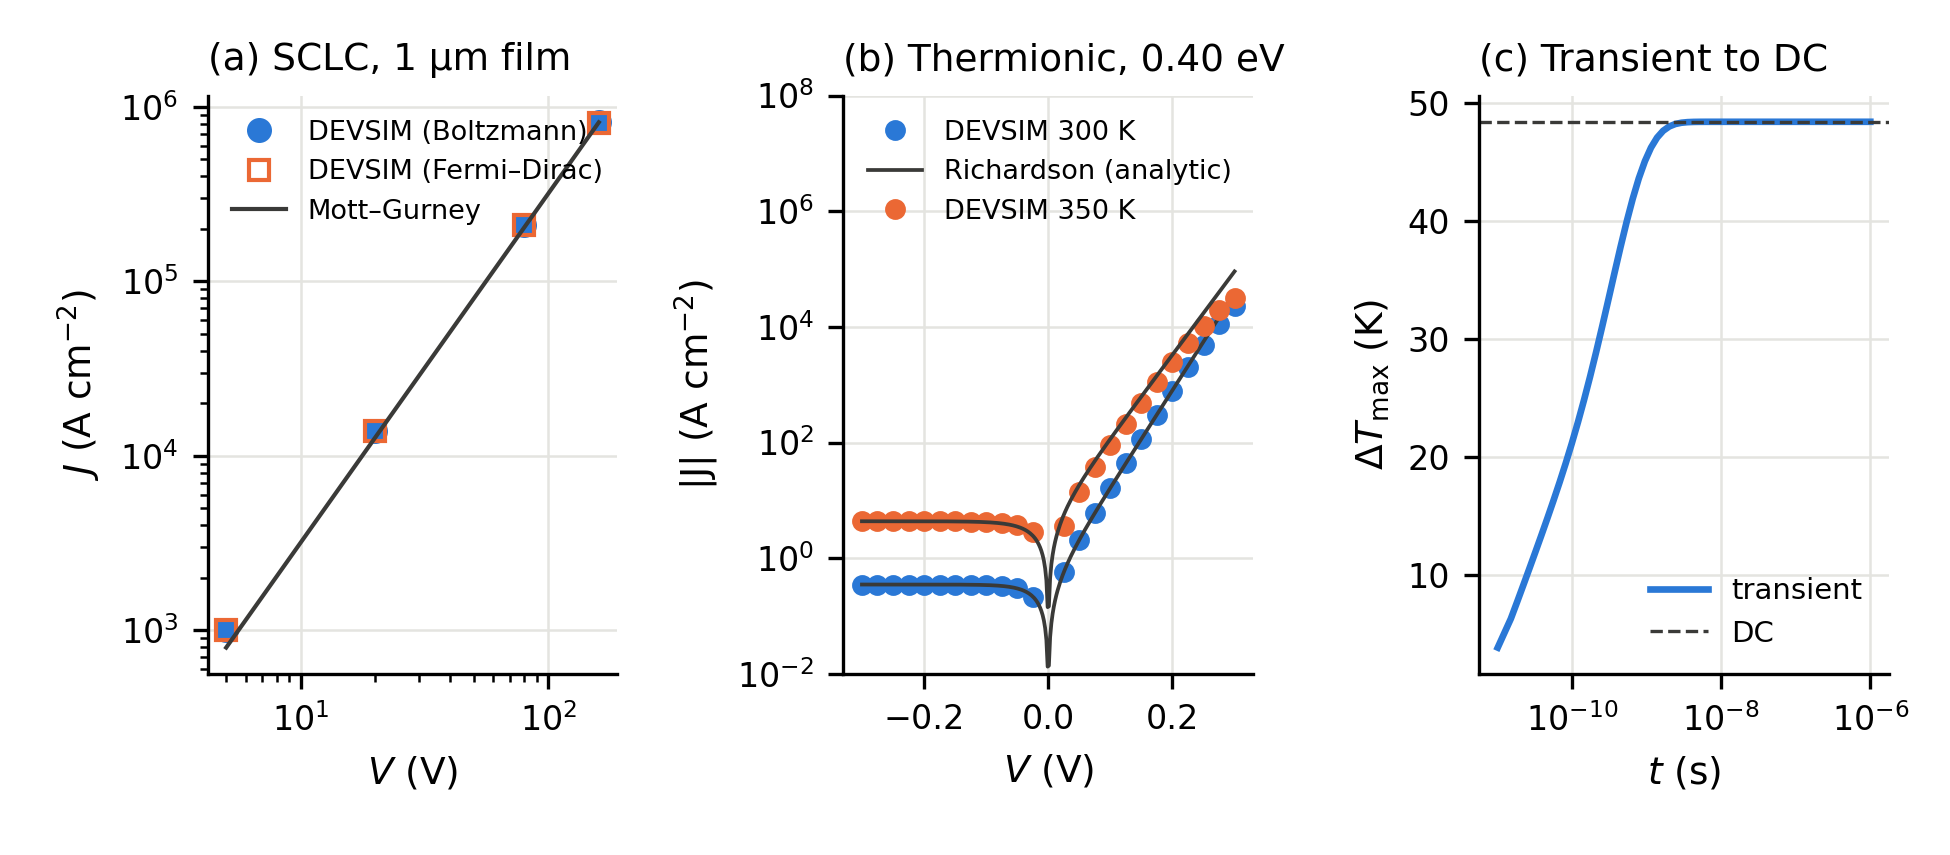
\includegraphics[width=0.96\textwidth]{fig1_verification.png}
\caption{Verification. (a) Mott--Gurney law with Boltzmann and Fermi--Dirac statistics. (b) Thermionic emission at 300 and 350~K. (c) Transient heating of a gated edge device stepped to 1~V (tunnelling off), approaching the DC solution.}
\label{fig:ver}
\end{figure}

\subsection{Numerical benchmark on Au/MoS$_2$}
\label{sec:cal}
No measurements of hole injection into p-InSe exist that could fix the interface parameters. We therefore use a different, well-characterised system only as a numerical benchmark of the solver, contact and tunnelling implementation: the best-characterised metal/2D contact, ultra-high-vacuum Au on 4.5-nm MoS$_2$ with a 90-nm SiO$_2$ back gate \cite{refenglish}. The measured quantities at $n=10^{13}$~cm$^{-2}$ are $R_c=740$~\ohmum, $\rho_c\approx3\times10^{-7}$~$\Omega$\,cm$^2$ and $L_T\approx35$--40~nm at 300~K, and $\rho_c\approx1.5\times10^{-7}$~$\Omega$\,cm$^2$ and $L_T\approx20$~nm at 400~K. We keep the 0.15-eV electron barrier assumed in that work and use literature MoS$_2$ parameters, with an under-contact mobility of 35~cm$^2$/Vs scaling as $T^{-1.6}$. We fit a single parameter, $\mathcal{T}_{\rm vdW}$, to $R_c(300\,{\rm K})$ only. The quantities predicted out of sample are then $L_T(300\,\rm K)$ (from simulated $R_c(L_c)$ with $L_c=20$--200~nm), and $\rho_c$ and $L_T$ at 400~K.

\section{Results}
\subsection{Benchmark and out-of-sample test}
The fit gives $\mathcal{T}_{\rm vdW}=1.0$, at its physical bound: $R_c=731$~\ohmum\ against 740~\ohmum\ measured. With the literature barrier, nonlocal tunnelling carries 99.8\% of the injection, and no additional vdW tunnel barrier is needed. This is consistent with the clean interfaces of that study. Without further adjustment the model gives $L_T=34$~nm and $\rho_c=2.7\times10^{-7}$~$\Omega$\,cm$^2$ at 300~K: $\rho_c$ lies within the measured range, and $L_T$ is 3\% below the lower end of the measured 35--40~nm. At 400~K it predicts $\rho_c=2.0\times10^{-7}$~$\Omega$\,cm$^2$ (measured 1.5) and $L_T=29$~nm (measured $\approx$20, quoted uncertainty up to 50\%), with the measured direction of change for both (Fig.~\ref{fig:mos2}). The model underestimates how much $L_T$ shrinks with temperature. This is consistent with its temperature-independent barrier and no phonon-assisted injection. We take the agreement as validation of the contact and tunnelling implementation at the 10--40\% level. It is a check of the numerics only: MoS$_2$ has a different band structure, no strong anisotropy and no layer-dependent gap, so it does not validate the InSe parameters or the InSe-specific results.

\begin{figure}[!htbp]
\centering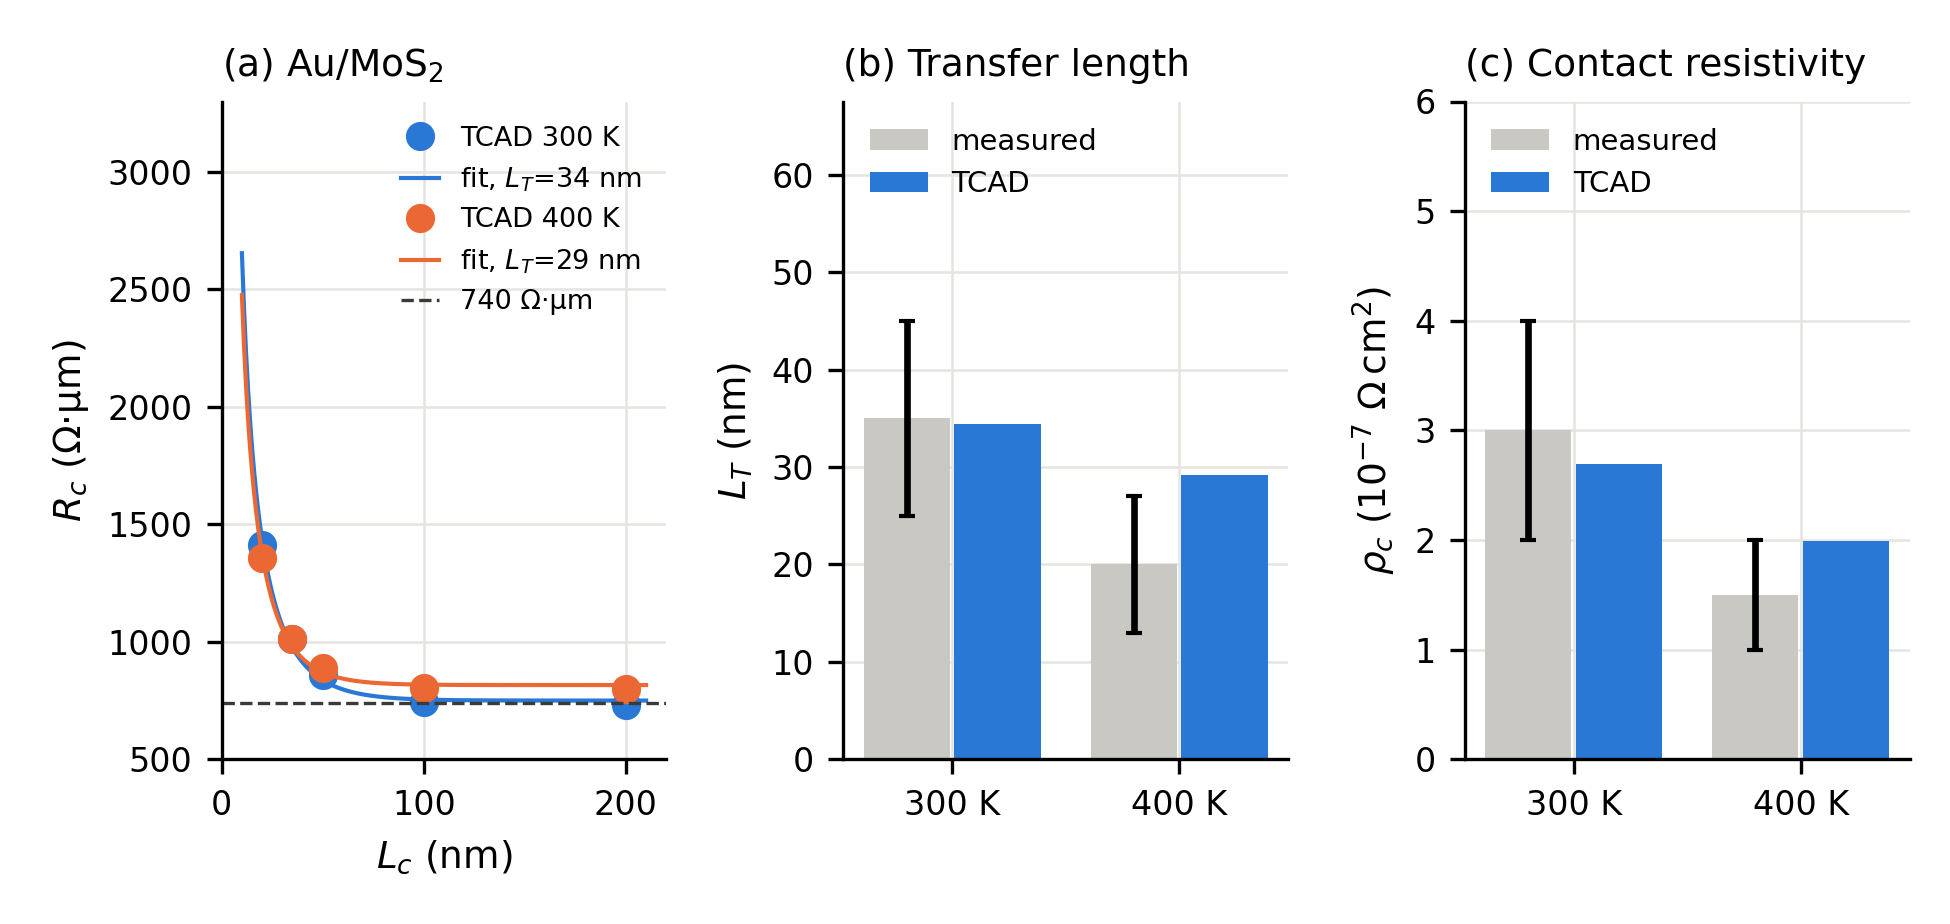
\includegraphics[width=0.96\textwidth]{fig8_mos2_calibration.png}
\caption{(a) Simulated $R_c(L_c)$ of Au/MoS$_2$ at 300 and 400~K with transmission-line fits. (b) Transfer length and (c) specific contact resistivity against the measurements of Ref.~\cite{refenglish}, with their quoted uncertainties. Only $R_c$ at 300~K was fitted; the 400~K values and $L_T$ are predictions.}
\label{fig:mos2}
\end{figure}

\subsection{Ungated InSe: work function, statistics and tunnelling}
\label{sec:res_ungated}
Without a gate (Fig.~\ref{fig:wf}), $R_{\rm tot}$ at 0.05~V falls exponentially with $\Phi_M$ down to $E_V=5.0$~eV. For 4.8~eV it is 1430~\ohmcm\ (edge), 5080~\ohmcm\ (top, 50~nm) and 11\,500~\ohmcm\ (top, 10~nm). With Fermi--Dirac statistics the resistance keeps decreasing for degenerate contacts: at 5.65~eV it is 5.4, 7.3 and 7.7~\ohmcm, a factor 2.1--2.6 below the Boltzmann result, which is clipped at $E_V$. Contacts carry 67\% (top, 50~nm) and 87\% (top, 10~nm) of $R_{\rm tot}$ at 4.8~eV, against 7.5\% for the edge. In the ungated, fully depleted film, nonlocal tunnelling carries 44\% of the edge-contact current and lowers its resistance by 13\% relative to pure thermionic emission. For top contacts it carries $\leq$8.5\% and lowers resistance by 2--6\%. For the edge contact the local $\Gamma(F)$ model recovers only a fifth of this reduction (2.3\% vs 12.6\%), because only nonlocal injection bypasses the diffusion-limited part of the barrier; for top contacts, where injection is limited by the interface, the two models differ by about 1\%.

\begin{figure}[!htbp]
\centering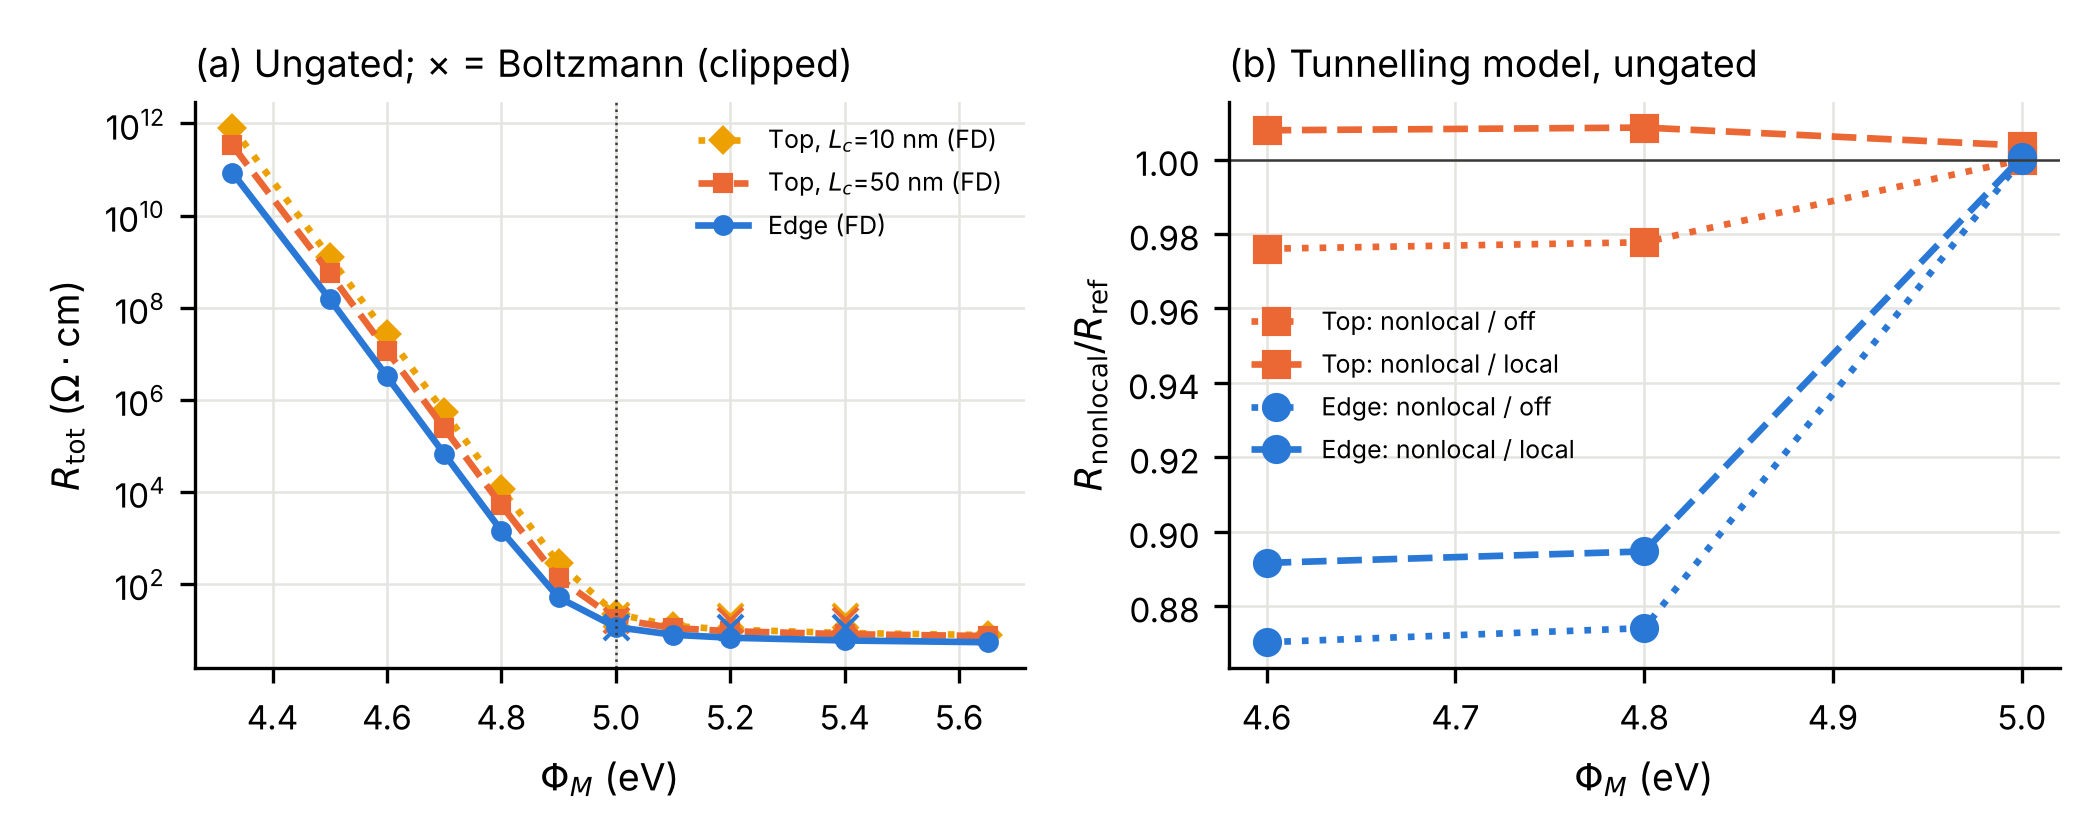
\includegraphics[width=0.96\textwidth]{fig3_wf_statistics_tunnelling.png}
\caption{Ungated devices. (a) $R_{\rm tot}$ versus $\Phi_M$ with Fermi--Dirac statistics (lines) and Boltzmann statistics clipped at $E_V$ ($\times$). (b) Ratio of nonlocal-tunnelling resistance to the no-tunnelling and local-$\Gamma$ models.}
\label{fig:wf}
\end{figure}

\subsection{Anisotropy and top-contact length}
Out-of-plane transport limits top contacts (Fig.~\ref{fig:aniso}). Lowering $\mu_\perp/\mu_\parallel$ from 1 to 0.002 doubles the top-contact resistance at 4.8~eV (3920$\to$7990~\ohmcm\ for 50~nm; 8270$\to$16\,700~\ohmcm\ for 10~nm), whereas edge contacts are unaffected. The edge advantage at 4.8~eV therefore grows from 64\% (isotropic) to 72\% (baseline) and 82\% ($r_\mu=0.002$). The top-contact resistance saturates for $L_c\gtrsim50$--100~nm, which indicates transfer lengths of a few tens of nanometres. Thermal anisotropy matters little at this thickness: with $\kappa_\perp=0.76$ instead of 8.5~W/mK, the temperature rise of ungated devices at 1~V changes by less than 4\% (the gated operating point of Sec.~\ref{sec:heat} is more sensitive: 8--17\%).

\begin{figure}[!htbp]
\centering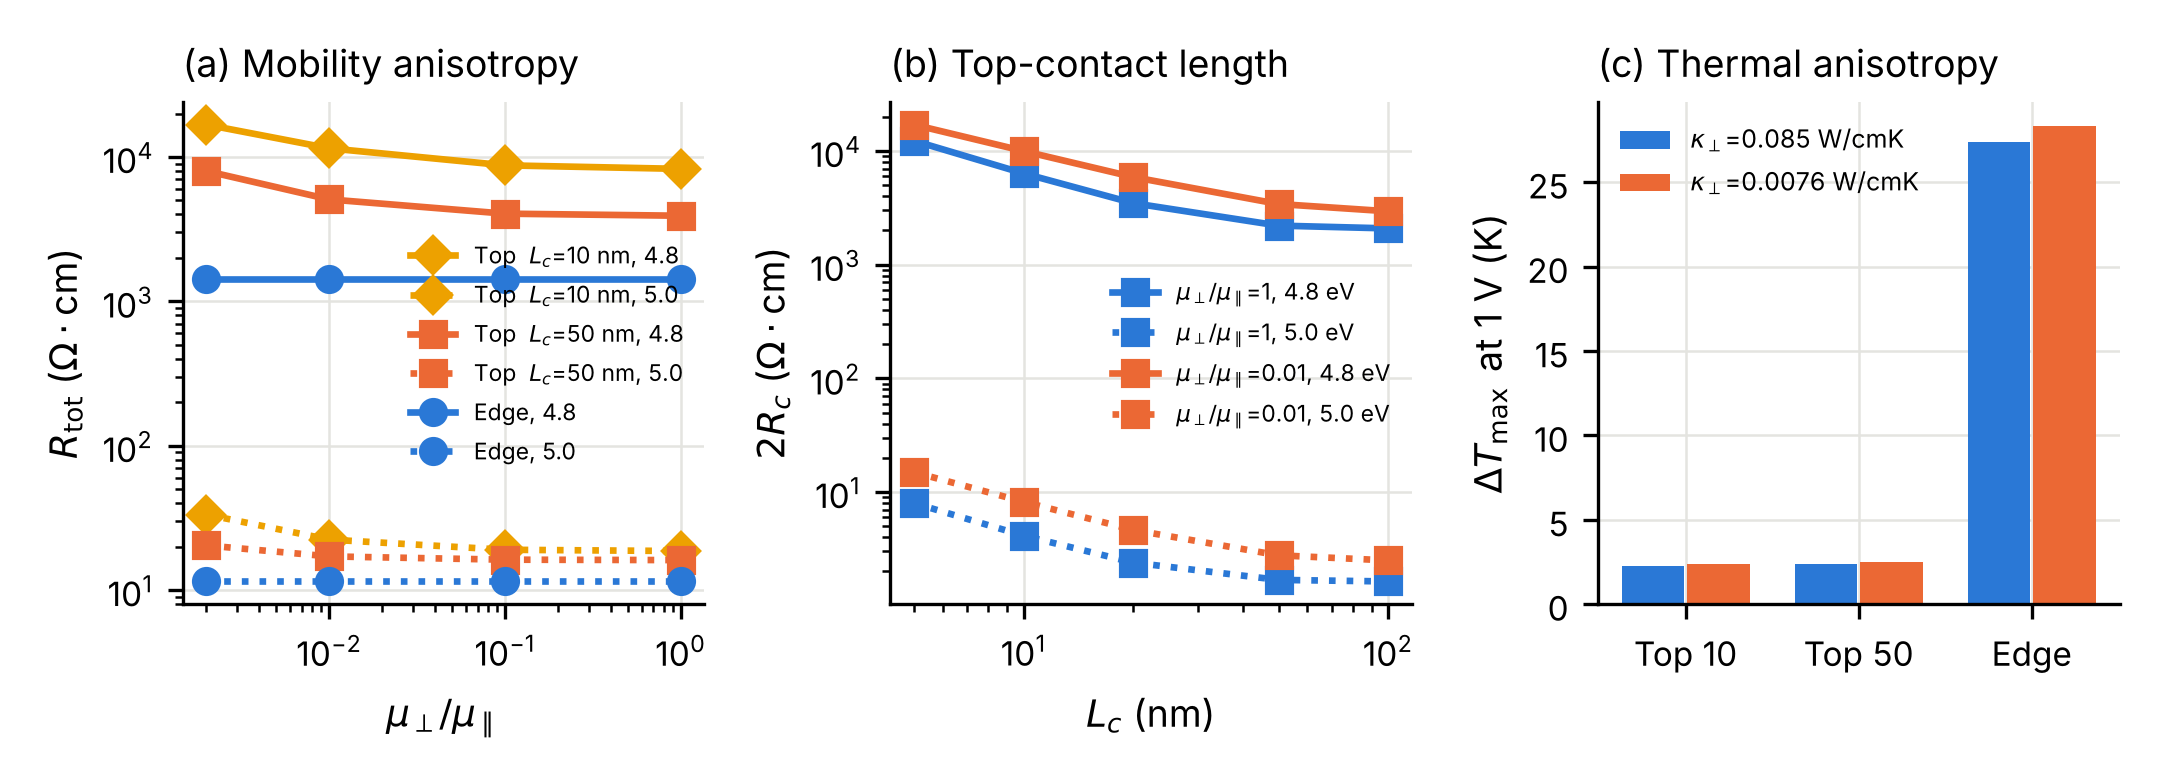
\includegraphics[width=0.96\textwidth]{fig4_anisotropy.png}
\caption{(a) $R_{\rm tot}$ versus out-of-plane/in-plane mobility ratio (colour: geometry; line style: $\Phi_M$). (b) $2R_c$ of top contacts versus contact length for two mobility ratios. (c) Peak temperature rise of ungated devices at 1~V for isotropic and measured $\kappa_\perp$.}
\label{fig:aniso}
\end{figure}

\subsection{Pinning: can top contacts win?}
\label{sec:res_pin}
Edge contacts expose dangling bonds and may be more strongly pinned than vdW top contacts. Figure~\ref{fig:pin} varies $S_{\rm edge}$ with $S_{\rm top}=1$. Already at $S_{\rm edge}=0.7$ the edge contact is 180$\times$ more resistive than with $S_{\rm edge}=1$ at 4.8~eV ($2.6\times10^5$~\ohmcm), and 50$\times$ worse than the 50-nm top contact. It overtakes the top contact again only for metals with $\Phi_M\geq5.4$~eV. The geometric and vdW advantage of edge contacts is therefore smaller than the effect of a modest difference in pinning. Which geometry wins is decided by interface chemistry, and $S_{\rm edge}$ is the quantity experiments should measure first. This reversal applies to the ungated, barrier-limited contact. In the gated on state the edge contact keeps its advantage over a wide range of unequal pinning (Sec.~\ref{sec:uq}).

\begin{figure}[!htbp]
\centering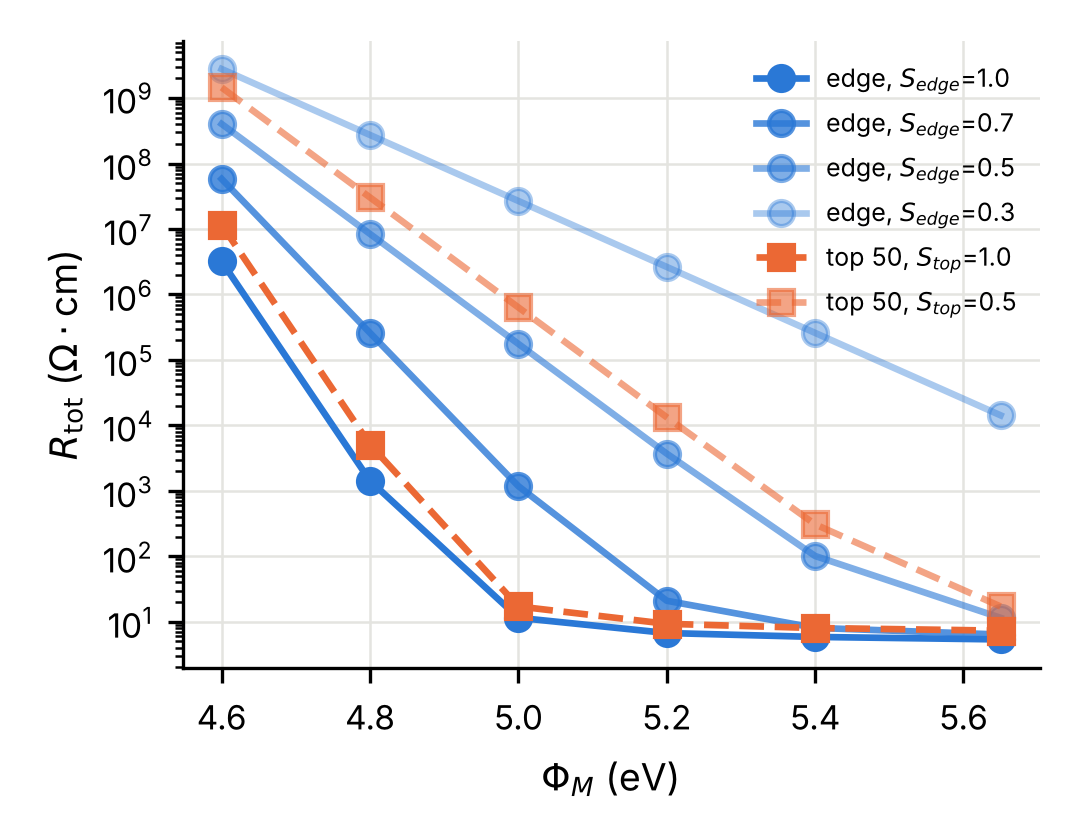
\includegraphics[width=0.55\textwidth]{fig5_pinning_top_vs_edge.png}
\caption{$R_{\rm tot}$ of edge contacts for $S_{\rm edge}=1$--0.3 and of 50-nm top contacts for $S_{\rm top}=1$ and 0.5 (ungated, 0.05~V).}
\label{fig:pin}
\end{figure}

\subsection{Measured pinning and literature band alignment}
\label{sec:measured}
Fermi-level pinning has been measured for InSe. Chen \textit{et al.}\ \cite{refchen} extracted barriers for In, Ti, Cr and Pd contacts and found $S=0.05\pm0.02$ for direct metal/InSe contacts, with the pinning level about 0.3~eV below $E_C$; a one-layer oxide interlayer raised $S$ to $0.5$. Hybrid-functional calculations for ideal, defect-free interfaces give $S=0.18$ with metal-induced gap states pinning $E_F$ about 0.58~eV above $E_V$ \cite{refguo}. We simulated Ti, Cr, Au, Pd and Pt (4.33--5.65~eV) for these three cases and for $S=1$, with $\chi=4.6$~eV and $S_{\rm top}=S_{\rm edge}$, and swept the hole barrier directly from 0 to 1~eV (Fig.~\ref{fig:measured}). The on state is $V_G=-3$~V at $V_D=0.05$~V.

With the measured direct-contact pinning every metal gives $\phi_{Bp}=1.05$--1.12~eV and an electron barrier of only about 0.3~eV. Direct metal contacts to InSe are therefore electron-injecting, which agrees with the n-type behaviour of most InSe transistors, and an ungated device conducts electrons rather than holes. Under a negative gate, holes are injected almost entirely by tunnelling ($\geq$99.9\%), and the edge on-state resistance is $5.2\times10^3$~\ohmcm\ for Pt and $1.2\times10^4$~\ohmcm\ for Ti, only 2.4$\times$ apart for a 1.3-eV range of work function. The choice of metal hardly matters.

With the calculated ideal pinning the barriers fall to 0.52--0.76~eV and the edge on-state resistance to 7.1~\ohmcm\ (Pt) to 123~\ohmcm\ (Ti). The measured oxide interlayer gives the same 0.52~eV for Pt, a 700$\times$ improvement over the direct Pt contact, but 0.79~eV for Pd and Au. Only an unpinned Pt contact reaches 0.25~eV and $R_{\rm tot}=0.51$~\ohmcm. Lowering the barrier, by depinning the interface or by choosing a high-work-function metal once it is depinned, is therefore the first lever for p-type InSe; geometry is the second.

The geometry lever becomes stronger, not weaker, as the barrier rises (Fig.~\ref{fig:measured}b). The ratio of top- to edge-contact on-state resistance is 4.1 at $\phi_{Bp}=0$, 14 at 0.2~eV, 35 at 0.4~eV, 51 at 0.6~eV, 74 at 0.8~eV and 150 at 1.0~eV. At high barriers the current must tunnel, and the edge contact tunnels in-plane with the gate field, while the top contact must tunnel vertically through the vdW gap and the slow out-of-plane path. Without tunnelling the resistance rises by $5\times10^2$ (edge) and $3\times10^2$ (top) at 0.2~eV and by $5\times10^7$ and $8\times10^6$ at 0.6~eV, so a thermionic contact model would declare any InSe hole contact unusable. Gated runs that did not converge are omitted. The hole current there is expected to be small, but this was not verified. They are the top contacts with $\phi_{Bp}\geq1.07$~eV (direct pinning except Pt; Ti and Cr with $S\geq0.5$) and the runs without tunnelling at 0.8--1.0~eV. For the measured direct pinning the top/edge ratio is therefore available only for Pt (170$\times$ at $\phi_{Bp}=1.05$~eV). The ungated resistance is not monotonic above $\phi_{Bp}\approx0.7$~eV because electron injection takes over.

As a consistency check against the measured electron barriers, we applied the same model to electron injection into an n-type film ($N_D=10^{16}$~cm$^{-3}$) with the measured direct pinning, for In, Ti and Pd contacts at 200--400~K (Fig.~\ref{fig:electron}a,b). At $V_G=0$ the Arrhenius barriers, from the slope of $\ln(I/T^2)$ against $1/T$, are 0.14--0.17~eV (edge) and 0.20--0.24~eV (top). They differ by at most 0.04~eV between metals across a 1-eV range of work function, in line with the weak metal dependence reported in Ref.~\cite{refchen}. They lie 0.06--0.16~eV below the input barrier of 0.30~eV because tunnelling contributes even without a gate, so barriers extracted this way are lower bounds. Above $V_G=+1$~V the Arrhenius slope turns negative because channel transport dominates. Figure~\ref{fig:electron}c shows the mesh convergence of the on-state resistances quoted in this section (Sec.~\ref{sec:ver}).

We then reproduced the measurement protocol of Ref.~\cite{refchen} as closely as its description allows: top contacts on 15-nm n-type InSe, a 300-nm SiO$_2$ back gate, In, Ti, Cr and Pd contacts, Arrhenius barriers from 300--400~K, and the reported pinning of the control ($S=0.05$, $\Phi_{\rm CNL}=4.9$~eV) and oxidized-monolayer ($S=0.5$, $\Phi_{\rm CNL}=5.2$~eV) contacts (Fig.~\ref{fig:chen}). Here $V_G=0$ is flat band. These pinning parameters are taken from Ref.~\cite{refchen}, so the barrier comparison tests the numerics and the extraction chain, not the InSe physics. The apparent pinning factors recover the inputs: 0.05 for the control and 0.53 (0.58 including In) for the oxide interlayer, against the reported 0.05 and 0.5. The Pd contact with the interlayer gives 0.54~eV, against about 0.57~eV in Ref.~\cite{refchen}. The In contact with the interlayer gives an Arrhenius slope of $-0.06$~eV, below the reported 65~meV. A pure $T^{-1.5}$ mobility alone gives $-0.10$~eV in this fit, so about 0.05~eV remains for the contact, close to the reported value, but a slope this small cannot resolve the contact barrier. The on-current is the one quantity not set by the inputs. It depends on the unreported channel length and on the electron mobility, which we first took as 1000~cm$^2$/Vs, a value for encapsulated films \cite{refband}, whereas Ref.~\cite{refchen} used InSe on SiO$_2$. At $V_G=80$~V and $V_D=1$~V with a 1-$\mu$m channel and $\mu_n=1000$~cm$^2$/Vs, the control device carries 19~$\mu$A/$\mu$m, against about 17--34~$\mu$A/$\mu$m inferred from the reported 3--6$\times$ ratio, and the oxide-interlayer device carries 187~$\mu$A/$\mu$m, against the reported 103~$\mu$A/$\mu$m. The ratio of 10$\times$ is then above the reported 3--6$\times$. It falls with the assumed mobility, because a device with a lower mobility is limited more by its channel and less by its contact (Fig.~\ref{fig:chen}b). At 100--200~cm$^2$/Vs the ratio is 4.2--5.6$\times$, inside the reported range, with 11--14~$\mu$A/$\mu$m (control) and 47--78~$\mu$A/$\mu$m (oxide), each within a factor of about two of the reported values. A 3-$\mu$m channel at 1000~cm$^2$/Vs gives 7.5$\times$. The mismatch at high mobility therefore does not show that the contact model overstates depinning. It shows that the on-current ratio of a channel-limited device is a weak test of the contact, and that the unreported mobility and channel length must be known before the measurement can calibrate the oxide-interlayer model.

\begin{figure}[!htbp]
\centering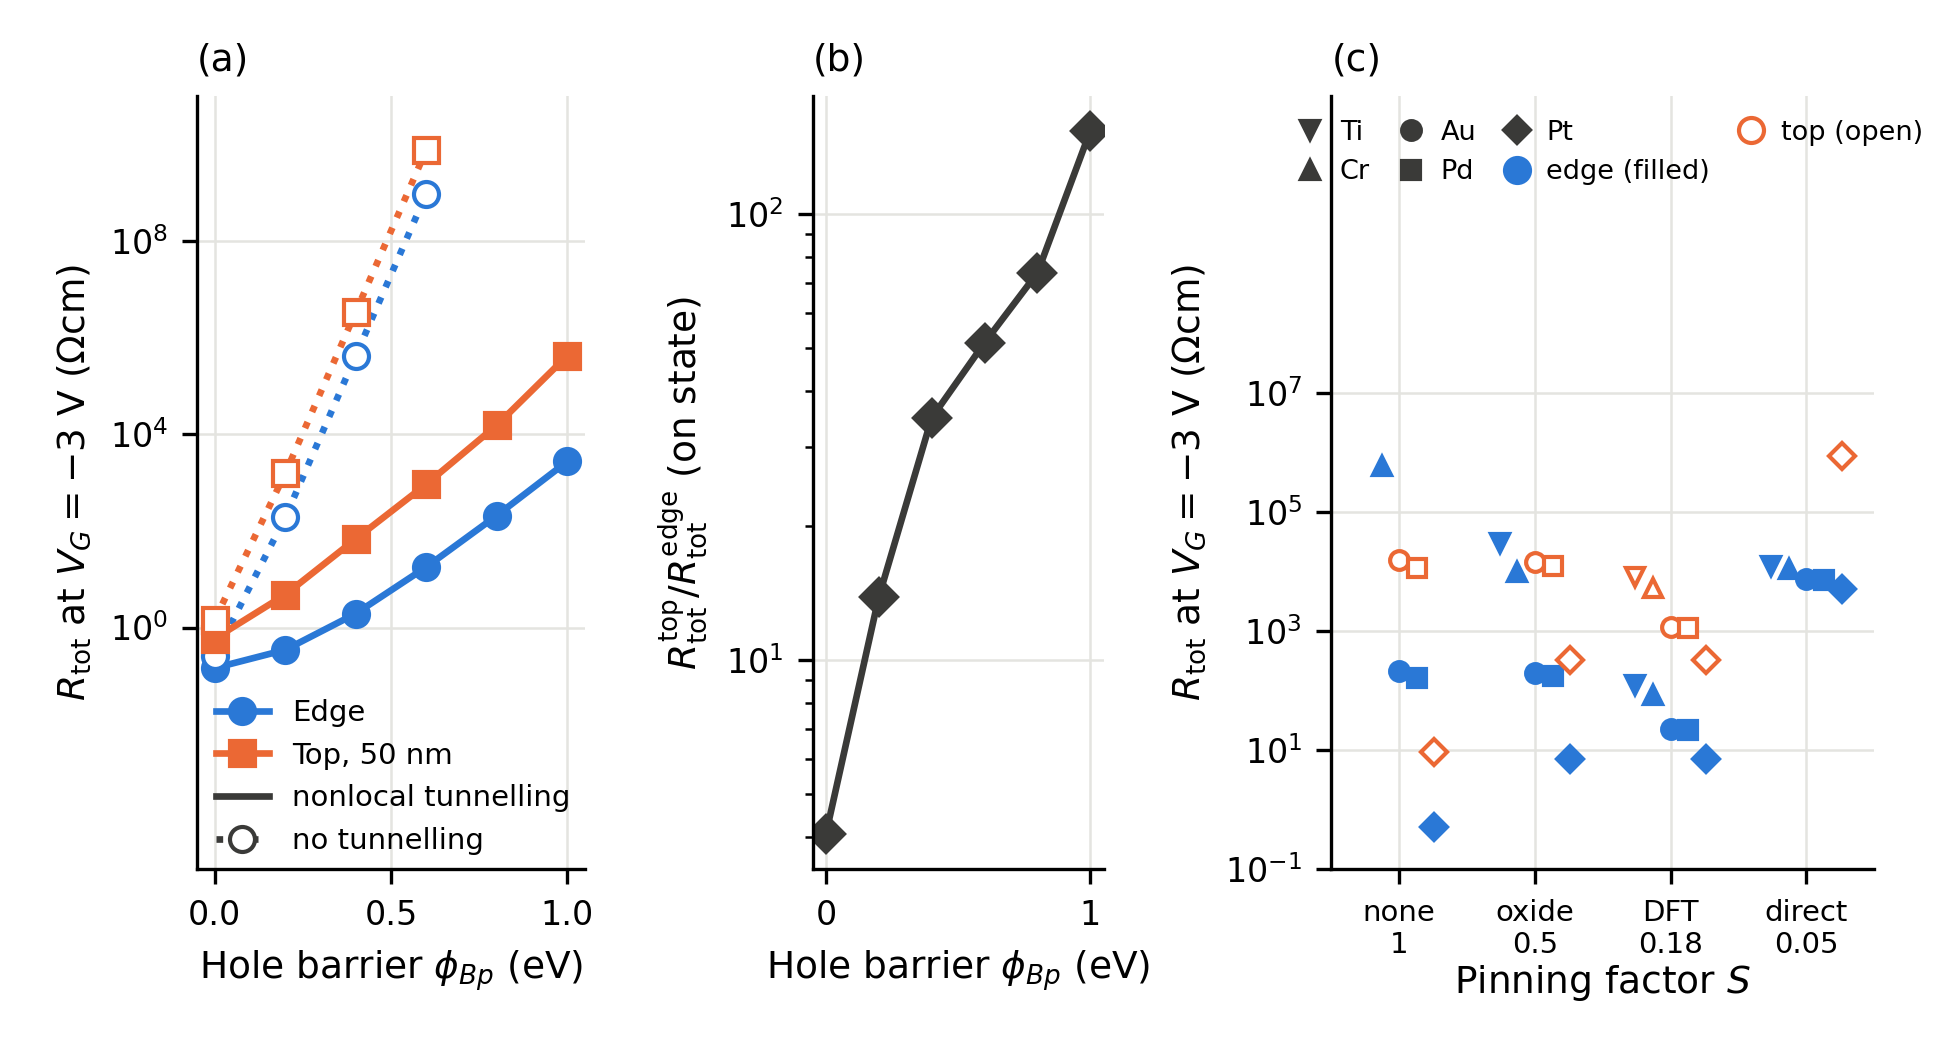
\includegraphics[width=0.96\textwidth]{fig12_measured_pinning.png}
\caption{Literature band alignment ($\chi=4.6$~eV, $E_V=5.90$~eV for 6 layers). (a) On-state $R_{\rm tot}$ ($V_G=-3$~V, $V_D=0.05$~V) versus hole barrier, with nonlocal tunnelling (solid) and without tunnelling (dotted). (b) Ratio of top- to edge-contact on-state resistance. (c) On-state $R_{\rm tot}$ for five metals and four pinning cases: no pinning; measured oxide interlayer and direct contact (M) \cite{refchen}; calculated ideal interface \cite{refguo}. Filled: edge; open: top, 50~nm. Missing points did not converge and were not determined.}
\label{fig:measured}
\end{figure}
\begin{figure}[!htbp]
\centering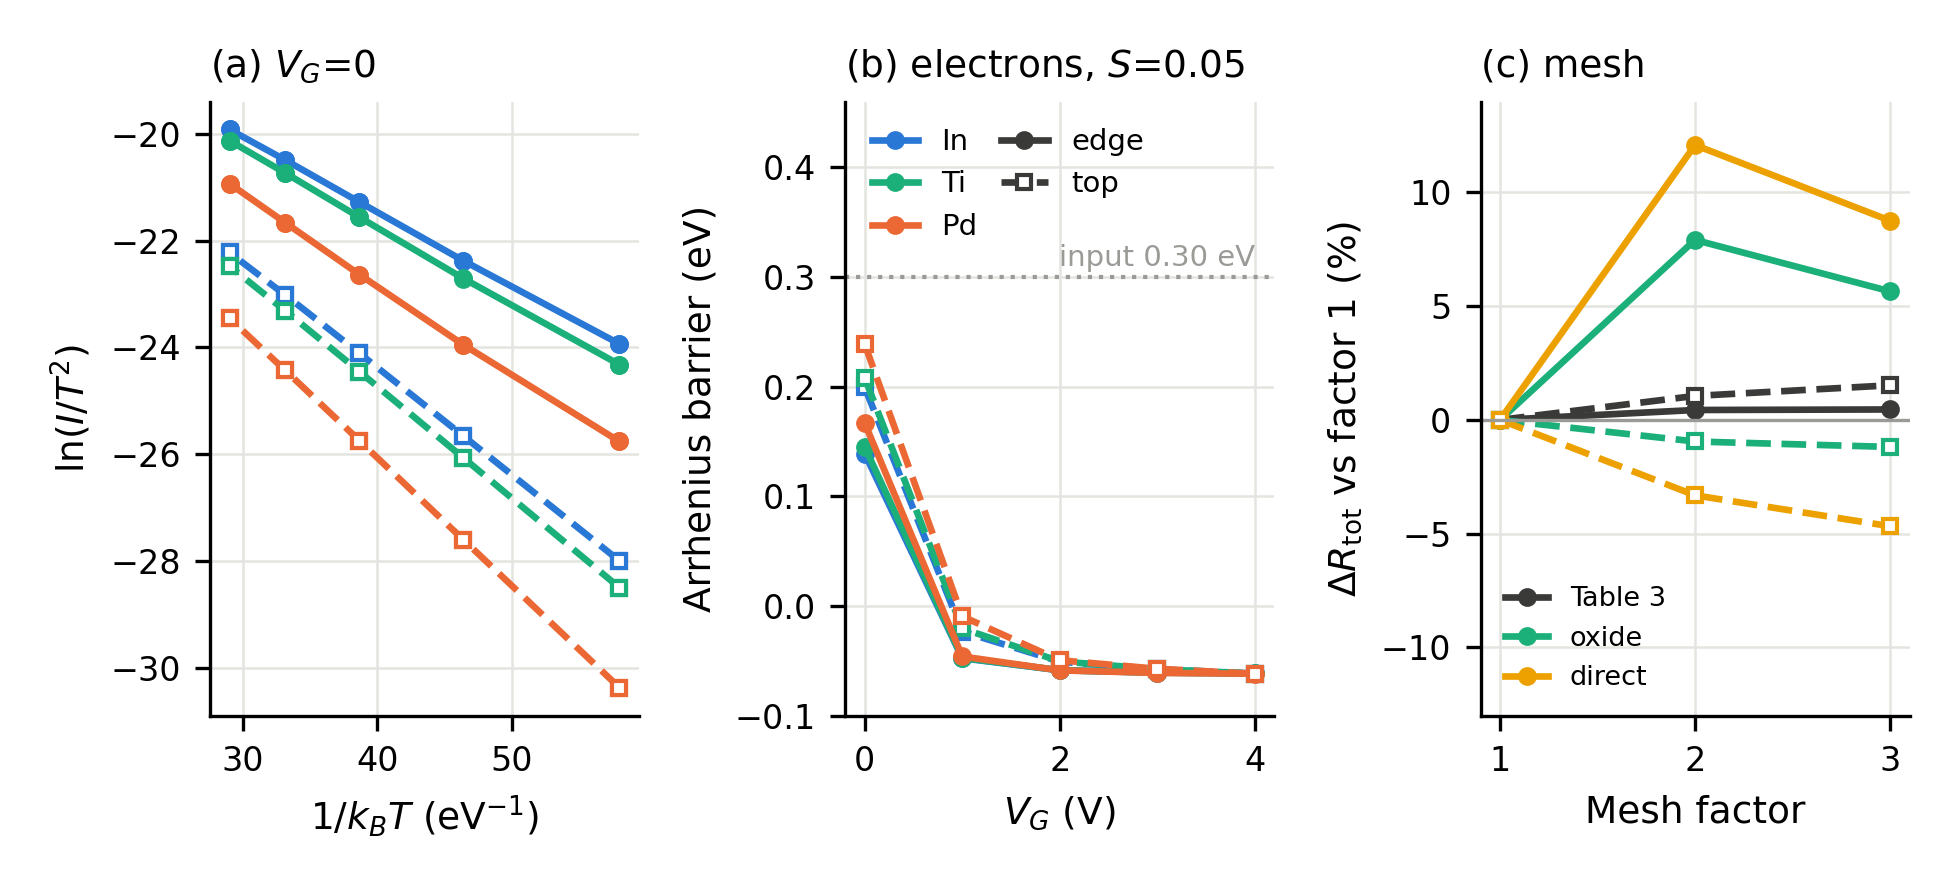
\includegraphics[width=0.96\textwidth]{fig15_electron_mesh.png}
\caption{(a) Arrhenius plots of electron injection at $V_G=0$ with the measured direct pinning ($S=0.05$, input barrier 0.30~eV) for In, Ti and Pd; filled: edge, open: top. (b) Arrhenius barrier versus $V_G$. (c) Change of $R_{\rm tot}$ with mesh factor for the Table~\ref{tab:therm} operating point and for the gated on state at the measured pinning (Pt, $V_G=-3$~V).}
\label{fig:electron}
\end{figure}

\begin{figure}[!htbp]
\centering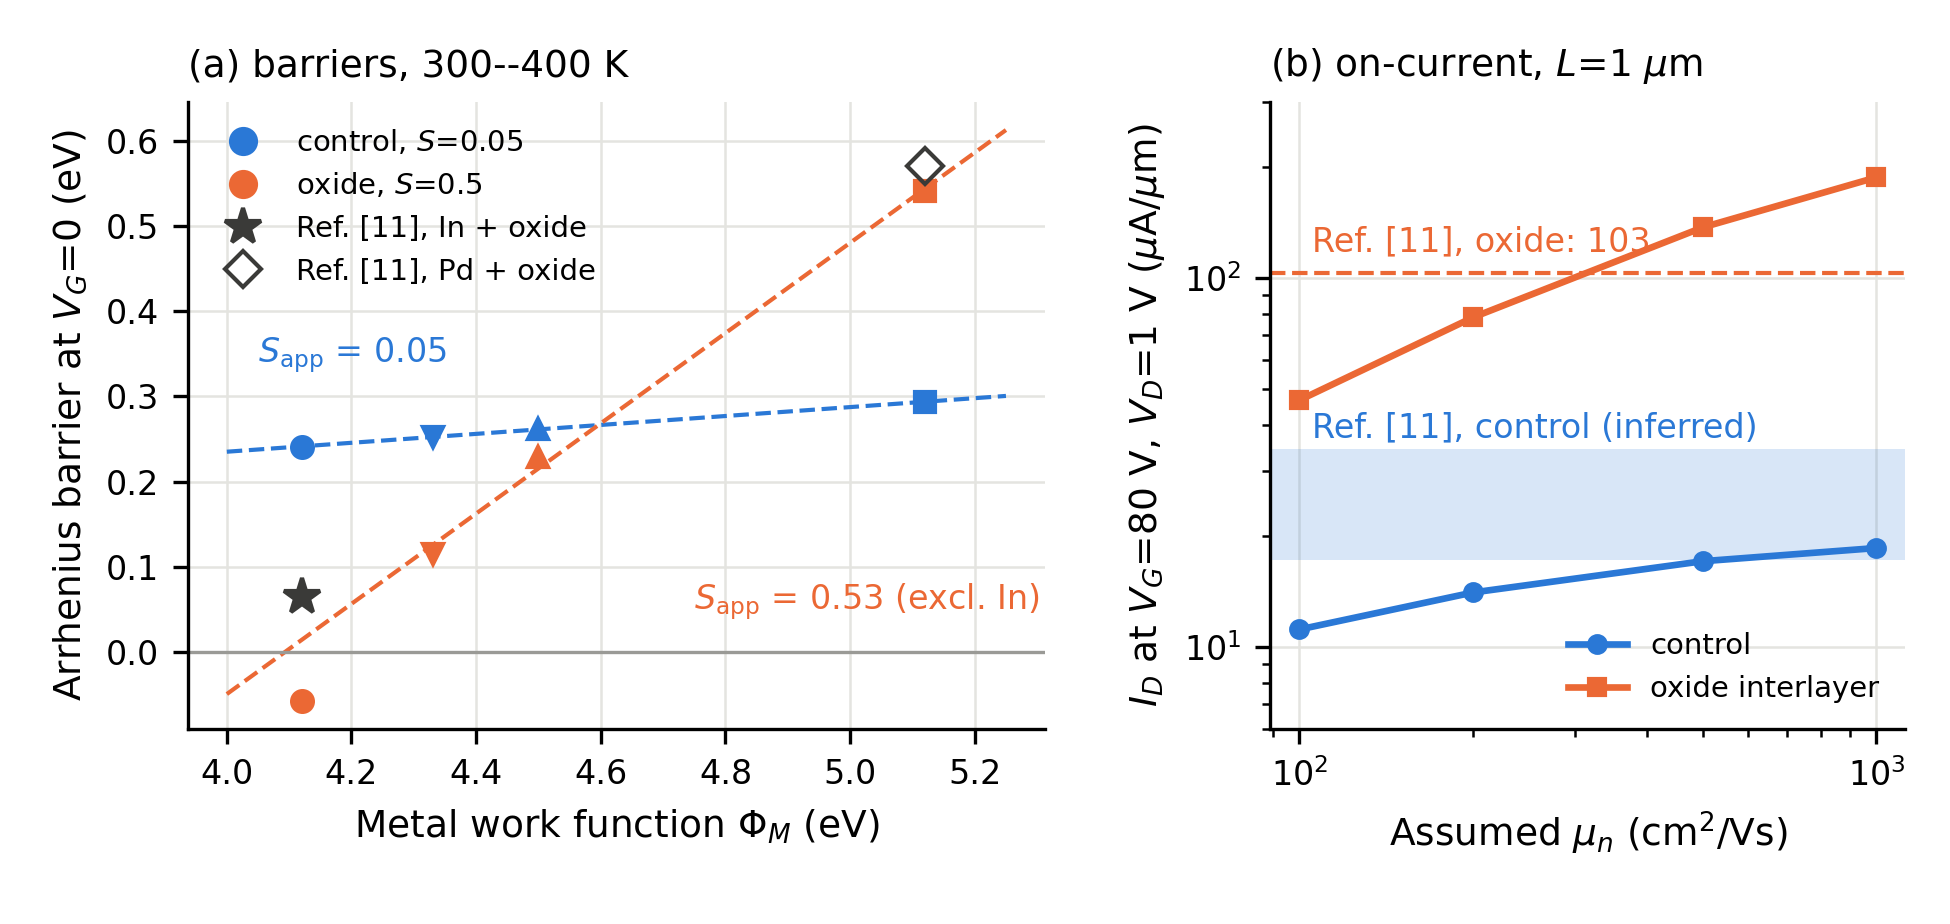
\includegraphics[width=0.96\textwidth]{fig16_chen2019.png}
\caption{Comparison with Ref.~\cite{refchen}. (a) Arrhenius barrier at flat band ($V_G=0$) for the control ($S=0.05$) and oxide-interlayer ($S=0.5$) contacts on 15-nm n-InSe; dashed lines are fits to the apparent pinning factor (the interlayer fit excludes In, whose slope is set by the channel). Reported values for the interlayer contacts are marked. (b) Drain current at $V_G=80$~V, $V_D=1$~V for an In contact with a 1-$\mu$m channel against the assumed electron mobility. The dashed line is the reported value of the oxide-interlayer device; the shaded band is the control current inferred from the reported 3--6$\times$ ratio. The channel length of the experiment is not reported.}
\label{fig:chen}
\end{figure}

\subsection{Gated Schottky-barrier p-FETs}
With the gate (Fig.~\ref{fig:gated}), both geometries switch with on/off ratios above $10^{12}$ between $V_G=+1$ and $-4$~V. At $\Phi_M=4.8$~eV the on-current at $V_D=0.05$~V and $V_G=-4$~V is 0.21~A/cm (edge) and 0.014~A/cm (top, 50~nm). Practically all of it is injected by tunnelling through the gate-thinned barrier: the no-tunnelling model gives 840$\times$ (edge) and 450$\times$ (top) less current, and the local $\Gamma(F)$ model 60$\times$ and 55$\times$ less. At 5.0~eV tunnelling still carries 80--83\% of the on-current; at 5.2~eV, where the contacts are degenerate, only 1--16\%. At 5.0~eV and $V_G=-4$~V the contact resistance is $R_c=86$~\ohmum\ (edge) against 2080~\ohmum\ (top), a factor of 24, while the channel resistances are nearly equal. The contact therefore limits the top-contacted transistor, and the channel limits the edge-contacted one.

\begin{figure}[!htbp]
\centering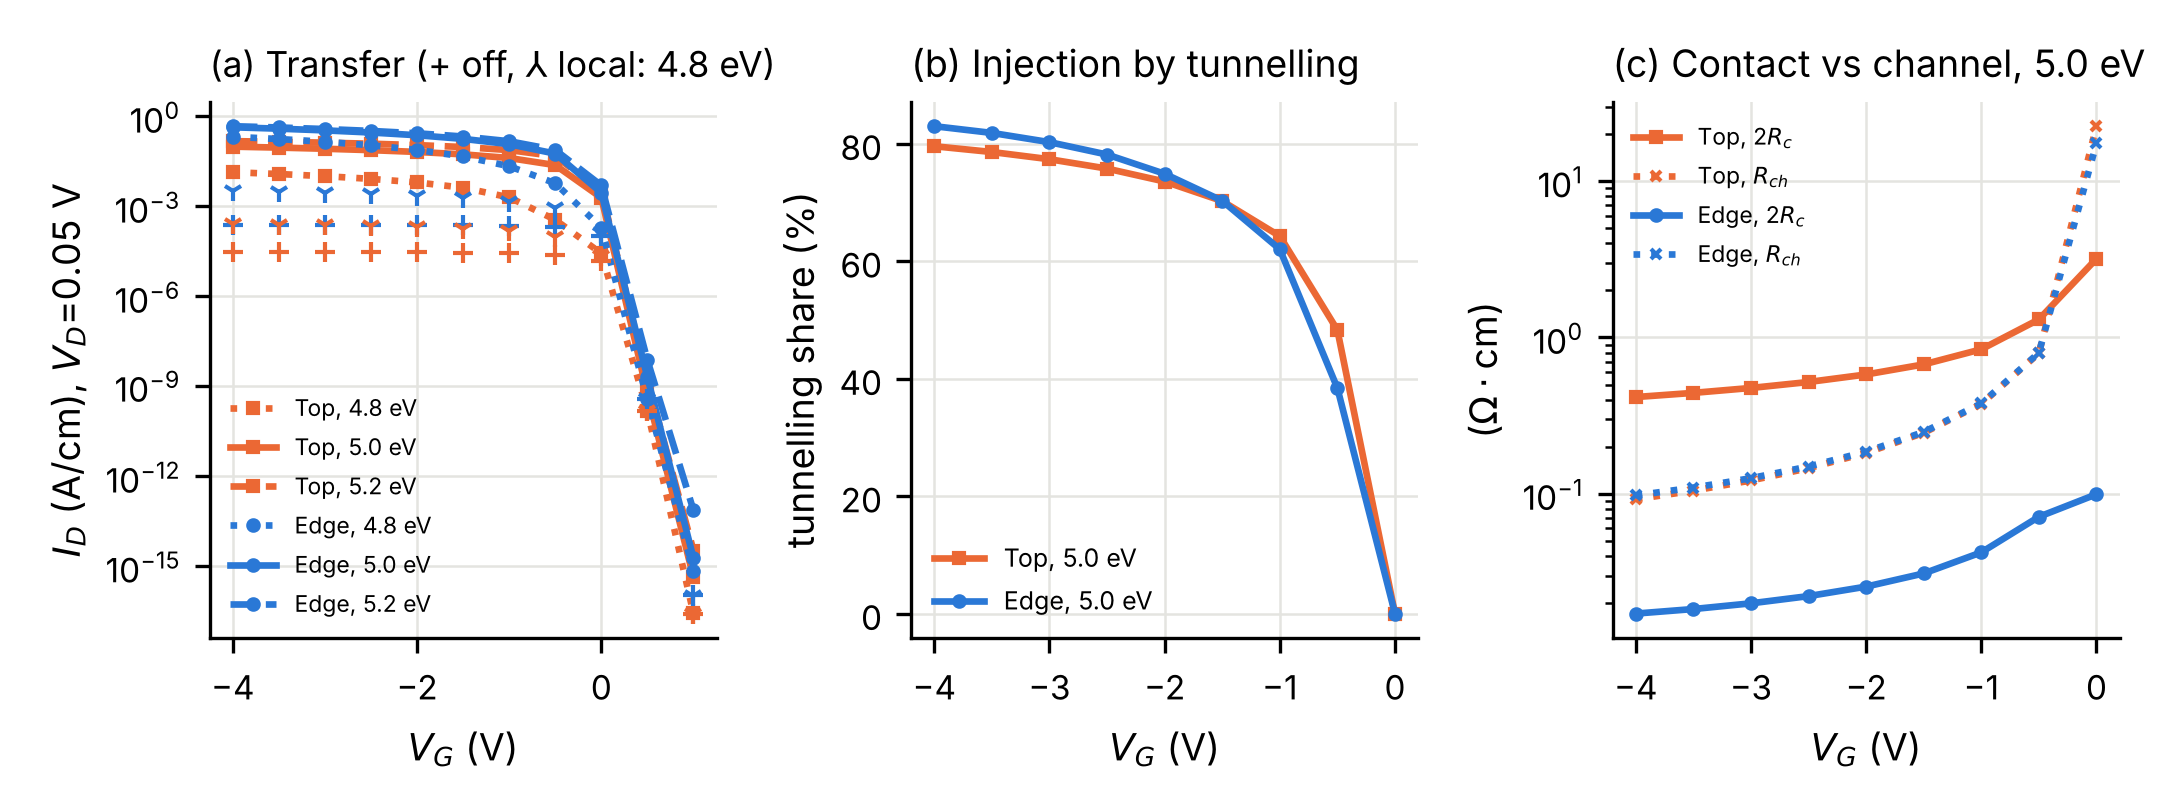
\includegraphics[width=0.96\textwidth]{fig6_gated_transfer.png}
\caption{Gated devices (10~nm SiO$_2$, $V_D=0.05$~V). (a) Transfer curves for the full nonlocal model (lines), with the no-tunnelling ($+$) and local-$\Gamma$ (Y-shaped symbols) models at 4.8~eV. (b) Share of the current injected by tunnelling. (c) Contact and channel resistance at 5.0~eV.}
\label{fig:gated}
\end{figure}

\subsection{Thickness}
\label{sec:thick}
Thinner films have larger band gaps and deeper valence bands (Fig.~\ref{fig:thick}a), so ungated resistances rise steeply below six layers. At 4.8~eV the edge-contact resistance rises from 242~\ohmcm\ (12 layers) to $1.1\times10^5$~\ohmcm\ (3 layers). In the gated on state ($\Phi_M=5.0$~eV, $V_G=-3$~V) the edge contact improves monotonically with thickness (0.197$\to$0.135~\ohmcm\ from 3 to 12 layers). The top contact instead has an optimum near four layers: 0.53~\ohmcm, rising to 1.55~\ohmcm\ at 12 layers. Beyond that thickness the vertical access through layers with low $\mu_\perp$ outweighs the shallower barrier (Fig.~\ref{fig:thick}b). These trends are robust to the band alignment and to the assumed 32\% valence-band share of the confinement shift (Fig.~\ref{fig:measuredalign}b,c). With the measured alignment and Pt contacts ($V_G=-3$~V) edge contacts again improve monotonically from 3 to 12 layers (oxide interlayer: 25$\to$4.5~\ohmcm), and top contacts have an optimum at five layers (interlayer, 207~\ohmcm) or six layers (direct pinning). Changing the valence-band share to 0.2 or 0.5 moves the optimum of the reference alignment between four and five layers.

\begin{figure}[!htbp]
\centering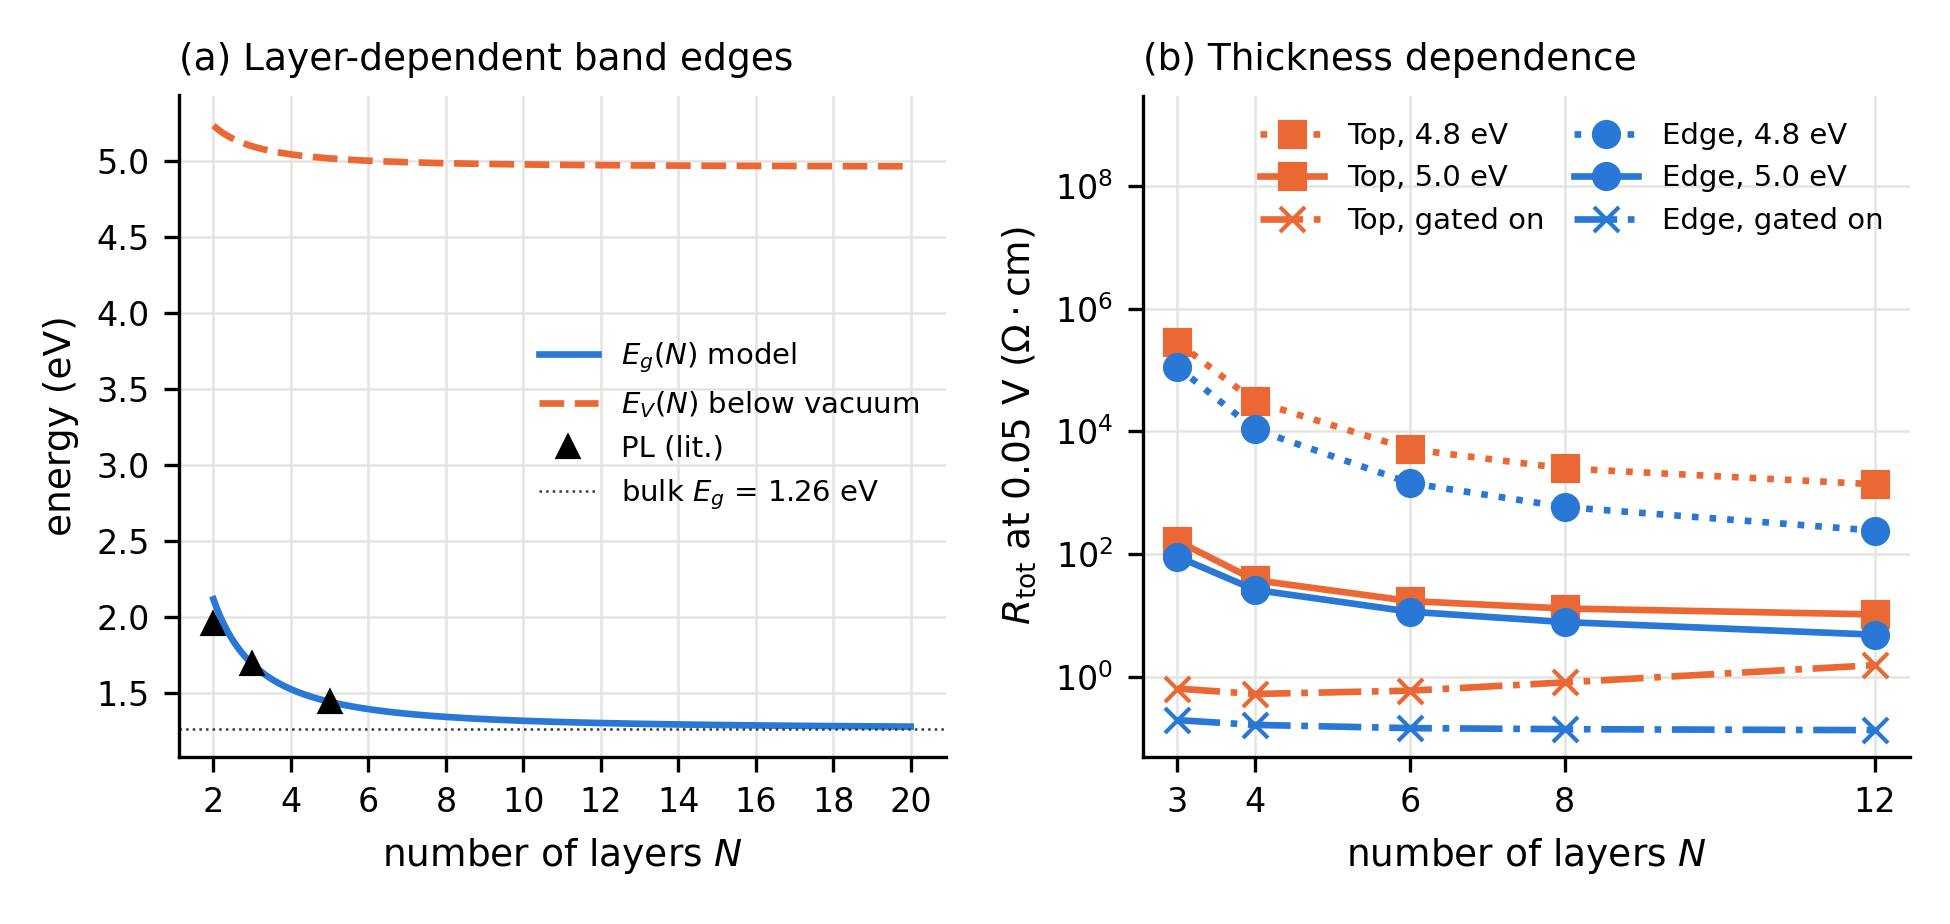
\includegraphics[width=0.96\textwidth]{fig2_thickness.png}
\caption{(a) Layer-dependent band gap and valence-band edge with photoluminescence data. (b) $R_{\rm tot}$ versus layer number, ungated and in the gated on state ($V_G=-3$~V, $\Phi_M=5.0$~eV).}
\label{fig:thick}
\end{figure}
\begin{figure}[!htbp]
\centering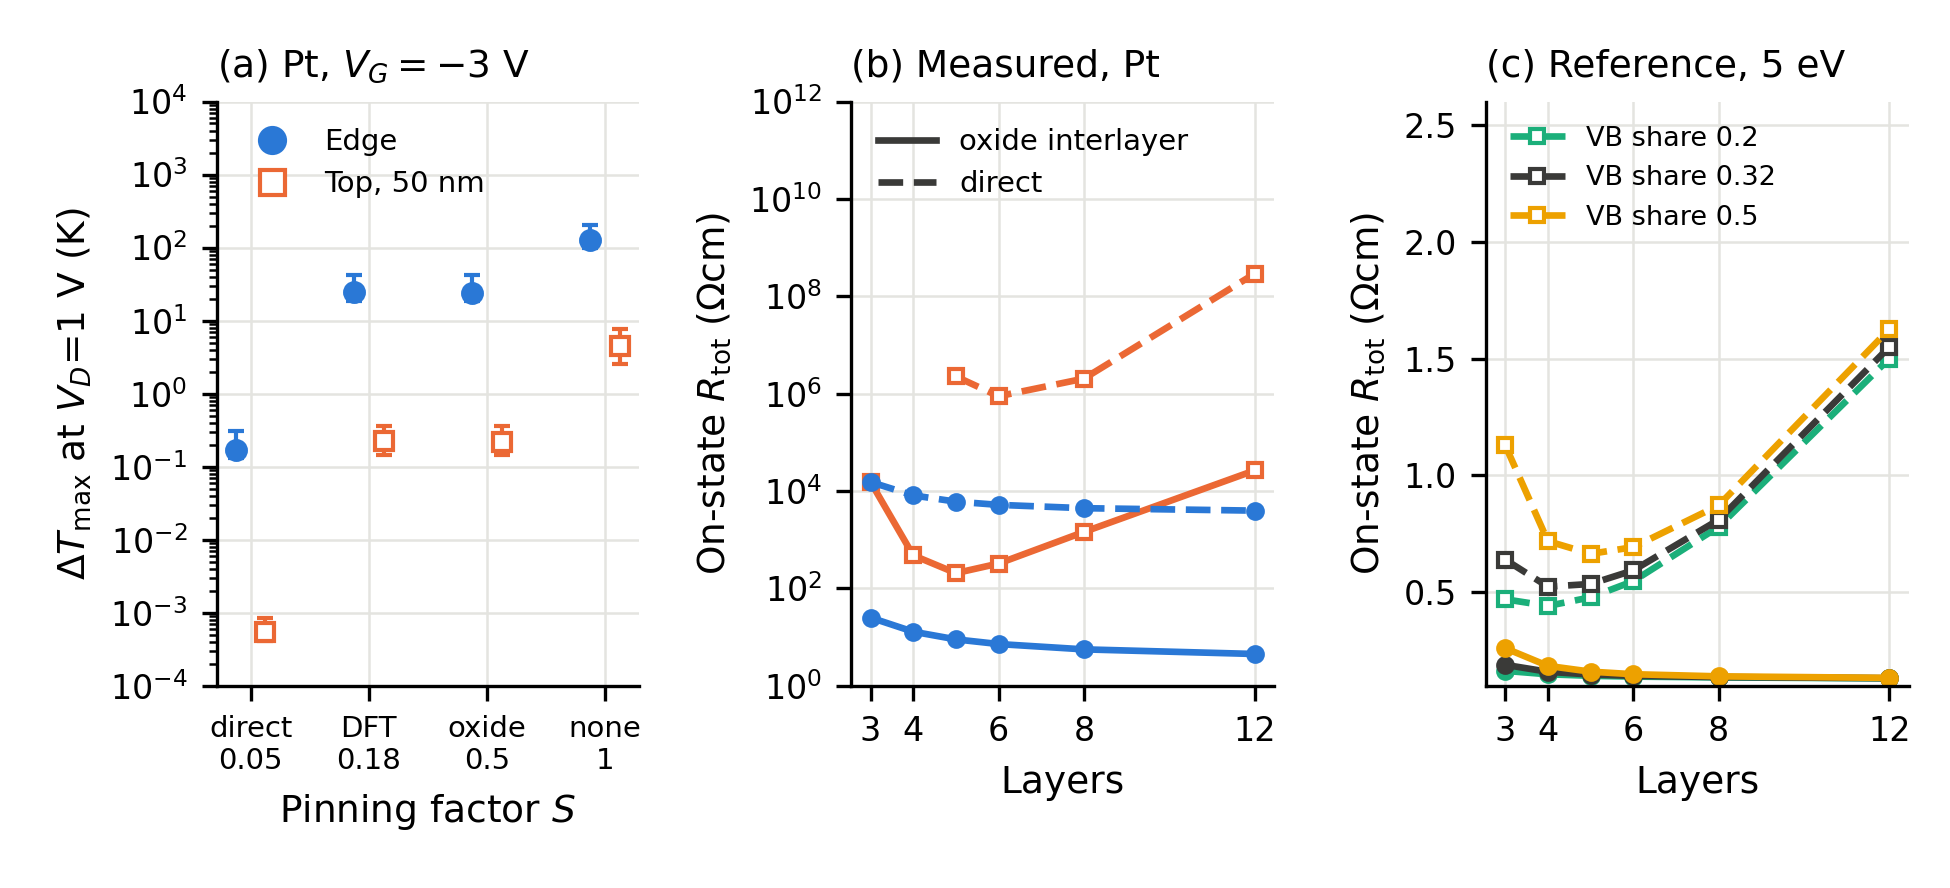
\includegraphics[width=0.96\textwidth]{fig14_measured_alignment.png}
\caption{Measured alignment. (a) Peak temperature rise at $V_D=1$~V, $V_G=-3$~V for Pt contacts and four pinning cases; bars span heat sinking through the metal (lower) and a three times larger $R_{\rm TBR}$ (upper). (b) On-state $R_{\rm tot}$ versus layer number for Pt with the oxide interlayer and direct pinning (missing top points did not converge). (c) Reference alignment ($\Phi_M=5.0$~eV, $S=1$) for valence-band shares of 0.2, 0.32 and 0.5. Filled: edge; open: top, 50~nm.}
\label{fig:measuredalign}
\end{figure}

\subsection{Self-heating}
\label{sec:heat}
Table~\ref{tab:therm} compares the geometries at the same gated operating point ($\Phi_M=5.0$~eV, $V_G=-2$~V). At $V_D=1$~V the edge-contacted device carries 3.7~A/cm and heats by 150~K; the 50-nm top contact carries 1.16~A/cm and heats by 24~K. Per unit power the edge device is also about twice as hot (41 vs 21~K\,cm/W), because its footprint on the oxide is a third of that of the top-contacted film. In the on state at $V_G=-3$~V (Fig.~\ref{fig:thermal}a) the edge device reaches about 490~K at 1~V, so its usable bias is thermally limited, not contact-limited. The two-dimensional maps in Fig.~\ref{fig:maps} show where the heat sits: in the top-contacted device the hottest point lies at the drain-side channel end on the contact side of the film, and the whole film stays within 24~K of ambient; in the edge-contacted device the film is 126--150~K hot everywhere and is coolest at the oxide interface, through which heat leaves to the substrate.

Table~\ref{tab:therm} uses the $S=1$ reference alignment, where $\Phi_M=5.0$~eV gives a hole barrier near zero. At the measured alignment (Pt, $V_G=-3$~V, $V_D=1$~V; Fig.~\ref{fig:measuredalign}a) self-heating depends on the pinning. Directly pinned contacts carry so little current that the edge device heats by only 0.2~K. With the oxide interlayer or the calculated ideal pinning ($\phi_{Bp}\approx0.52$~eV) the edge device heats by 24~K and the top-contacted one by 0.2~K. An unpinned Pt contact ($\phi_{Bp}=0.25$~eV) heats the edge device by 128~K (top: 4.4~K). Self-heating is therefore a concern only once the contacts are depinned. A three times larger $R_{\rm TBR}$ ($3\times10^{-8}$~m$^2$K/W) raises these rises by 58--73\%, and heat sinking through the metal lowers them by 22--23\%. Metal contacts are adiabatic in the baseline model, so the rises quoted are upper bounds. At the operating points of Table~\ref{tab:therm} the heat leaving the device equals $IV$ within 0.5\% (top) and 1.2--1.9\% (edge, 0.5 and 1~V). For the 150~K edge rise this is about 3~K, larger than the Peltier effect below, so temperatures are quoted to $\pm3$~K.

The individual heat terms matter at the 7--42\% level (Fig.~\ref{fig:thermal}b):
\begin{itemize}
\item Using bulk Joule heat only underestimates $\Delta T_{\max}$ by 7--8\% and misses 8--15\% of the dissipated power.
\item Measured out-of-plane conductivity, compared with isotropic $\kappa$, raises $\Delta T_{\max}$ by 8\% (edge) and 17\% (top).
\item Heat sinking through the metal contacts lowers $\Delta T_{\max}$ by 23\% (edge) and 42\% (top).
\item A ten times smaller thermal boundary resistance lowers it by 35--37\%.
\end{itemize}
Peltier heat changes $\Delta T_{\max}$ by only about 1~K but redistributes heat: it cools the hole-injecting contact and heats the collecting one (top, 1~V: source $+11.9$~K, drain $+21.6$~K with Peltier, against $+13.5$ and $+20.9$~K without). Temperature-dependent statistics change temperatures by less than 1\%. The lattice responds to a drain step within a few hundred picoseconds, with 63\% of the final rise at 0.20~ns (top) and 0.25~ns (edge) (Fig.~\ref{fig:thermal}c; this transient was simulated without tunnelling, so its amplitudes are smaller than in Table~\ref{tab:therm}). For pulses longer than a nanosecond the DC temperatures therefore apply.

\begin{table}[!htbp]
\centering
\caption{Gated operating points ($\Phi_M=5.0$~eV, $V_G=-2$~V, baseline thermal model). All quantities in a row refer to the same bias.}
\label{tab:therm}\small
\begin{tabular}{lcccccc}
\toprule
Geometry & $V_D$ (V) & $I_D$ (A/cm) & $IV$ (W/cm) & $\Delta T_{\max}$ (K) & $\Delta T_{\rm source}$ (K) & $\Delta T_{\rm drain}$ (K) \\
\midrule
Top, 50 nm & 0.5 & 0.618 & 0.309 & 5.9 & 3.5 & 5.6 \\
Top, 50 nm & 1.0 & 1.164 & 1.164 & 24.0 & 11.9 & 21.6 \\
Edge & 0.5 & 2.228 & 1.114 & 47.0 & 40.8 & 46.2 \\
Edge & 1.0 & 3.693 & 3.693 & 149.9 & 144.4 & 144.6 \\
\bottomrule
\end{tabular}
\end{table}


\begin{figure}[!htbp]
\centering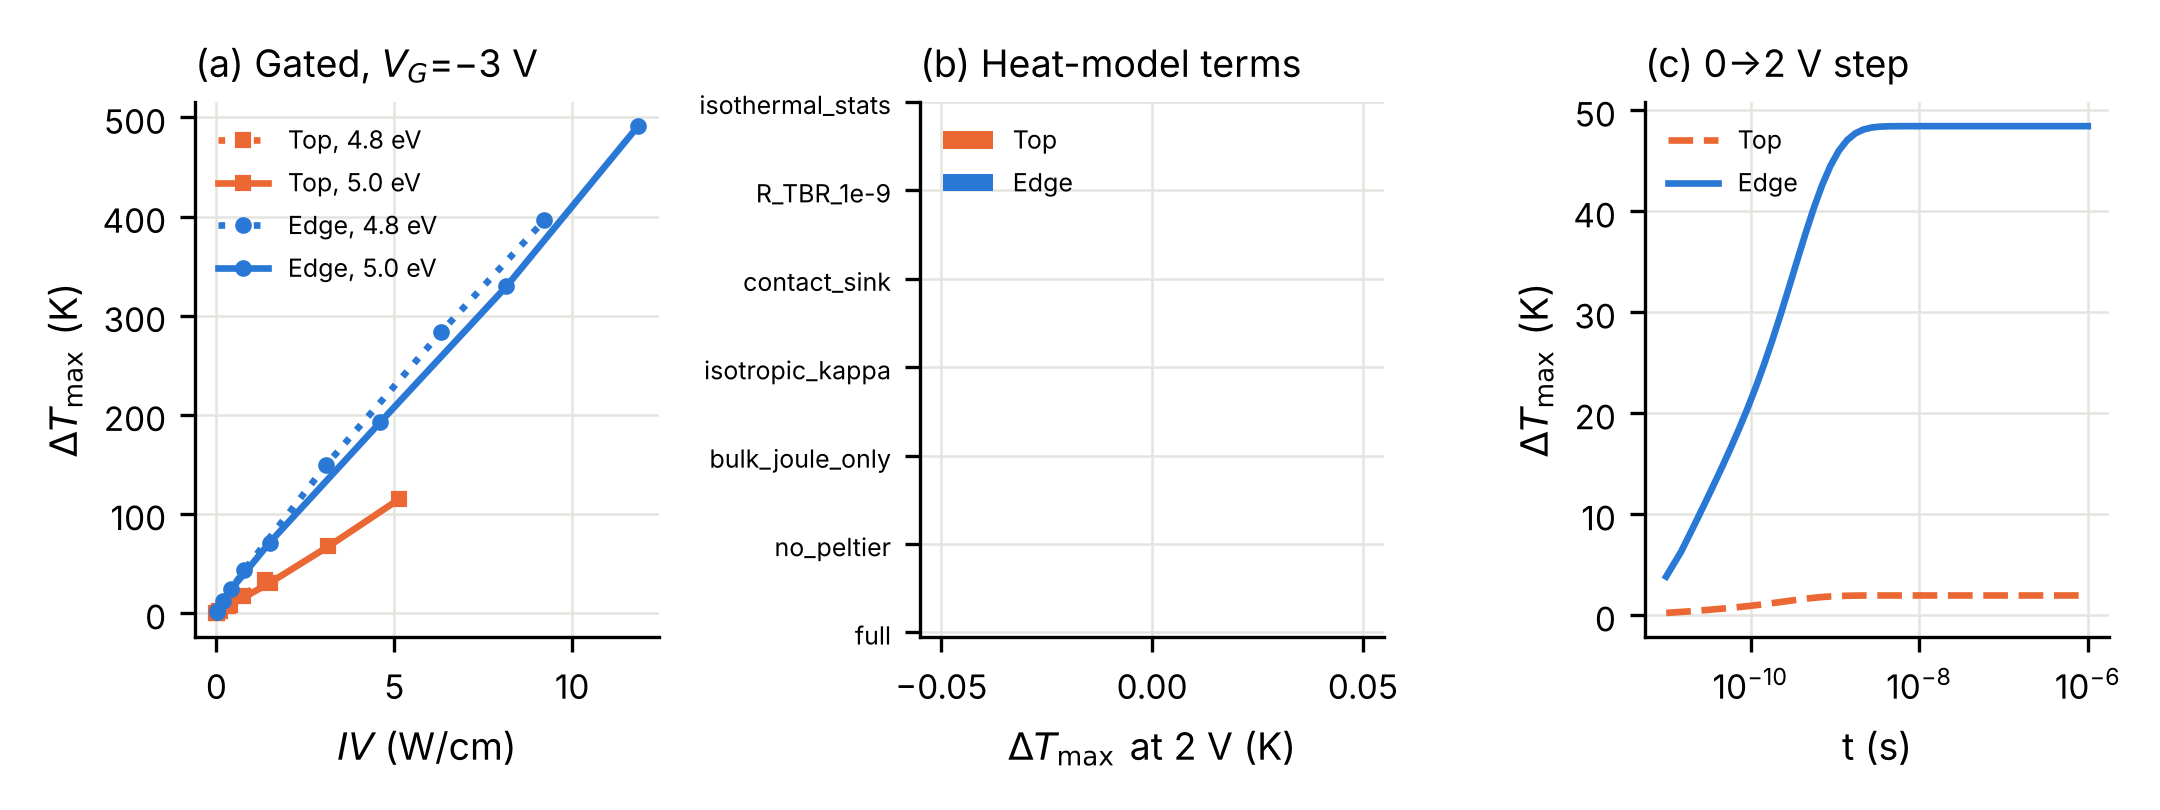
\includegraphics[width=0.96\textwidth]{fig7_thermal.png}
\caption{(a) Peak temperature rise versus dissipated power, gated on state. (b) Effect of each heat-model term at $V_D=1$~V, $V_G=-2$~V, $\Phi_M=5.0$~eV. (c) Response to a 0$\to$1~V drain step at $V_G=-2$~V, simulated without tunnelling (steady-state rises of 48~K and 2~K); only the time constant is used in the text.}
\label{fig:thermal}
\end{figure}

\begin{figure}[!htbp]
\centering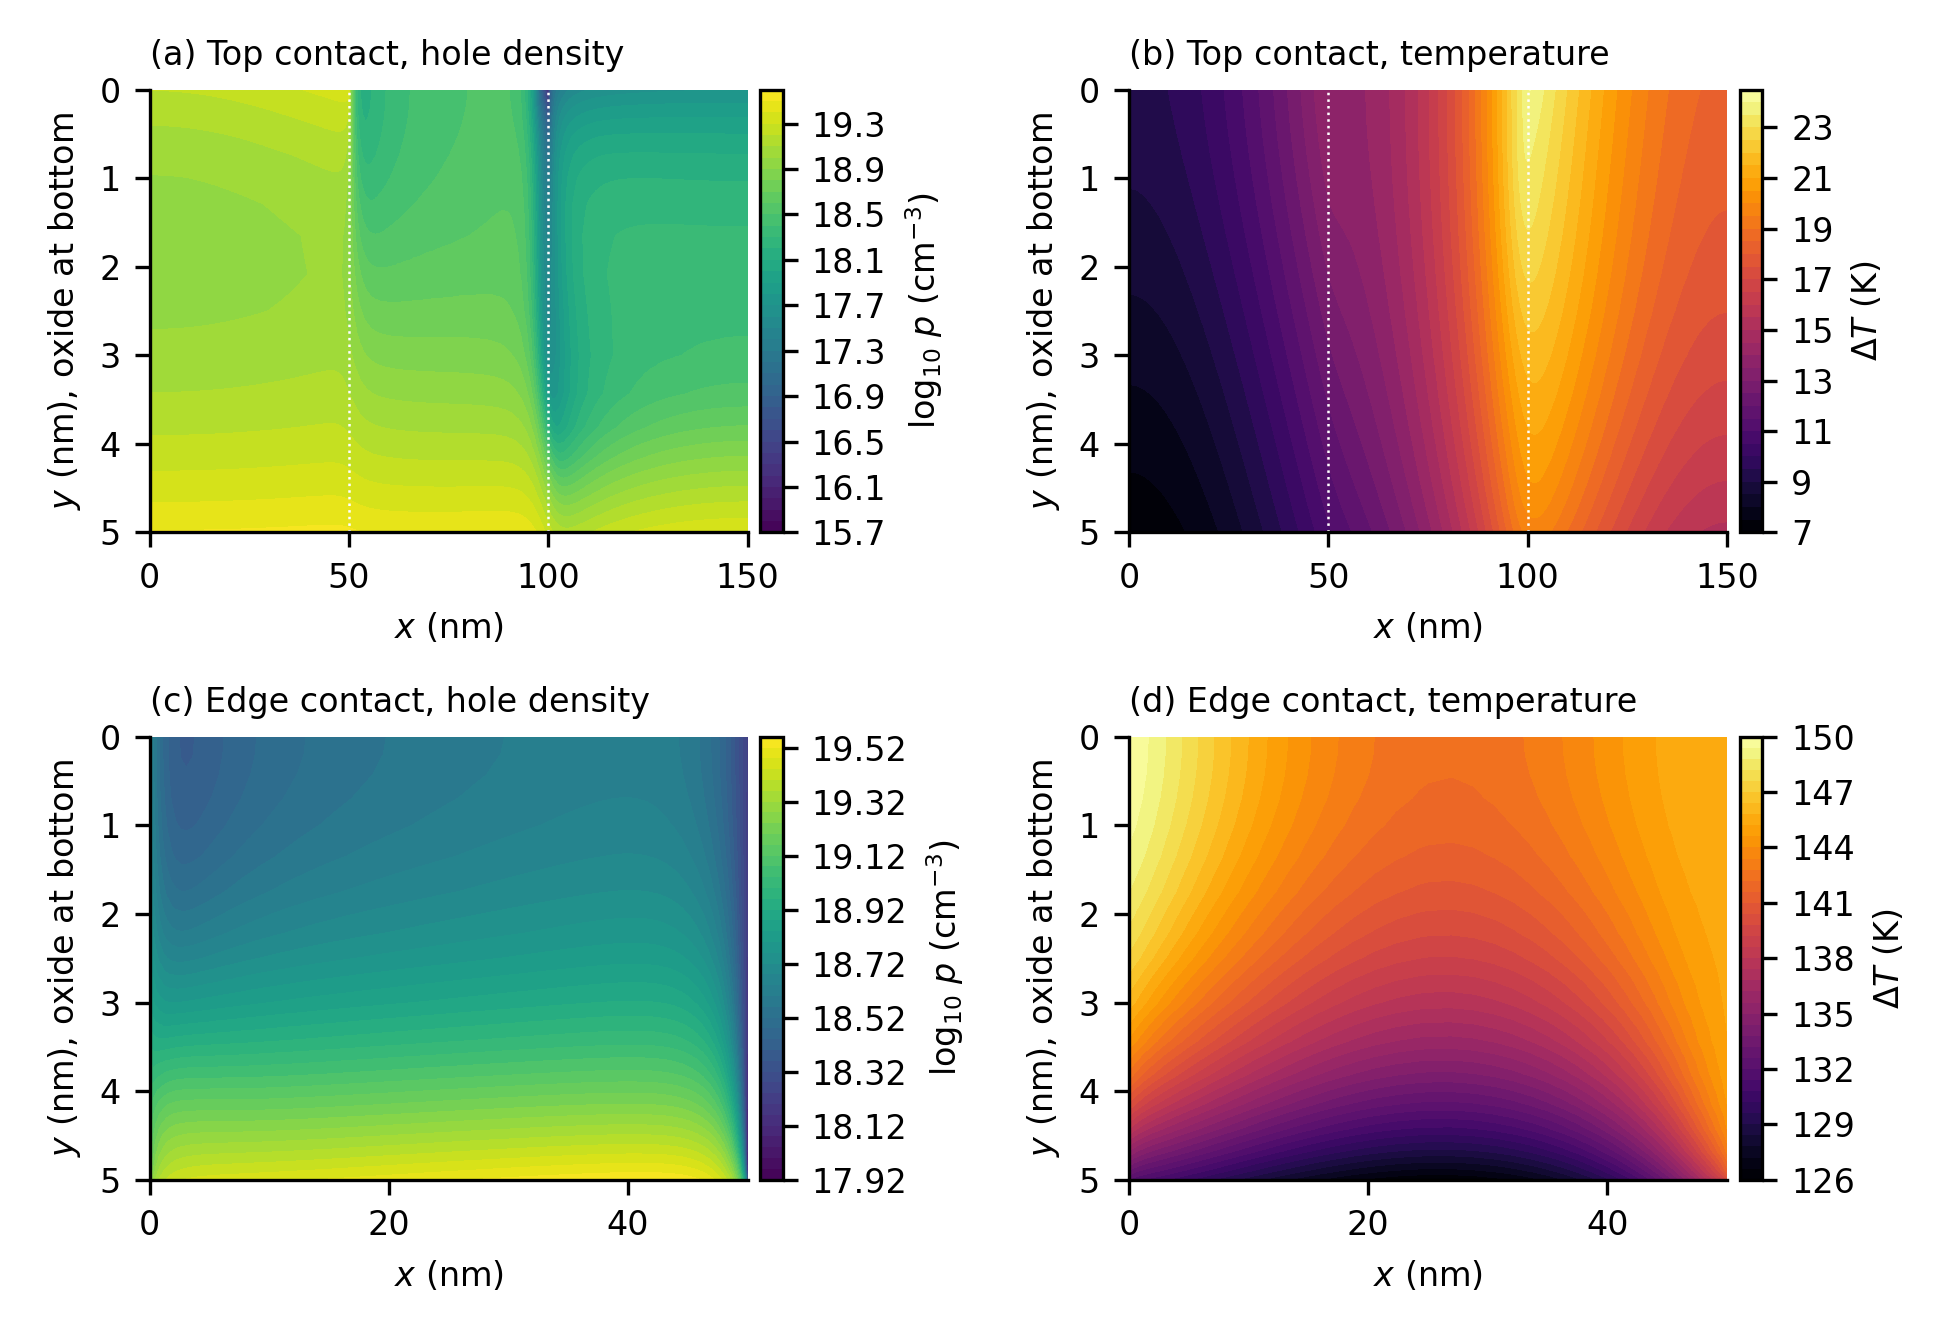
\includegraphics[width=0.96\textwidth]{fig11_field_maps.png}
\caption{Hole density and temperature rise of gated devices at $V_D=1$~V, $V_G=-2$~V, $\Phi_M=5.0$~eV (full model). The vertical axis is stretched: the film is 5~nm thick. The oxide interface is at the bottom ($y=5$~nm). Dotted lines in (a, b) mark the channel ends.}
\label{fig:maps}
\end{figure}

\subsection{Compact model}
For top contacts in the barrier-limited regime we compare a transmission-line model with the simulation. The model uses
\begin{itemize}
\item an interface resistivity $\rho_{\rm if}=V_t/(qv_R\mathcal{T}_{\rm vdW}p_{\rm eq})$;
\item a vertical access term $t/(2q\mu_\perp\bar p)$;
\item an under-contact sheet resistance $1/(q\mu_\parallel\bar pt)$;
\item $R_c=\sqrt{\rho R_{\rm sh}}\coth(L_c/L_T)$.
\end{itemize}
Over 120 cases ($\phi_{Bp}=0.05$--0.25~eV, $d_{\rm vdW}=0.2$--0.4~nm, $L_c=10$--100~nm, $r_\mu=1$ and 0.01) the fully predictive version, with $\bar p=p_{\rm eq}$, has a median error of 11\% and a 90th-percentile error of 33\% (Fig.~\ref{fig:compact}). Taking $\bar p$ from the simulation reduces the 90th percentile to 20\%. The compact model is therefore adequate for circuit-level estimates when tunnelling is weak, that is, without strong gating.

\begin{figure}[!htbp]
\centering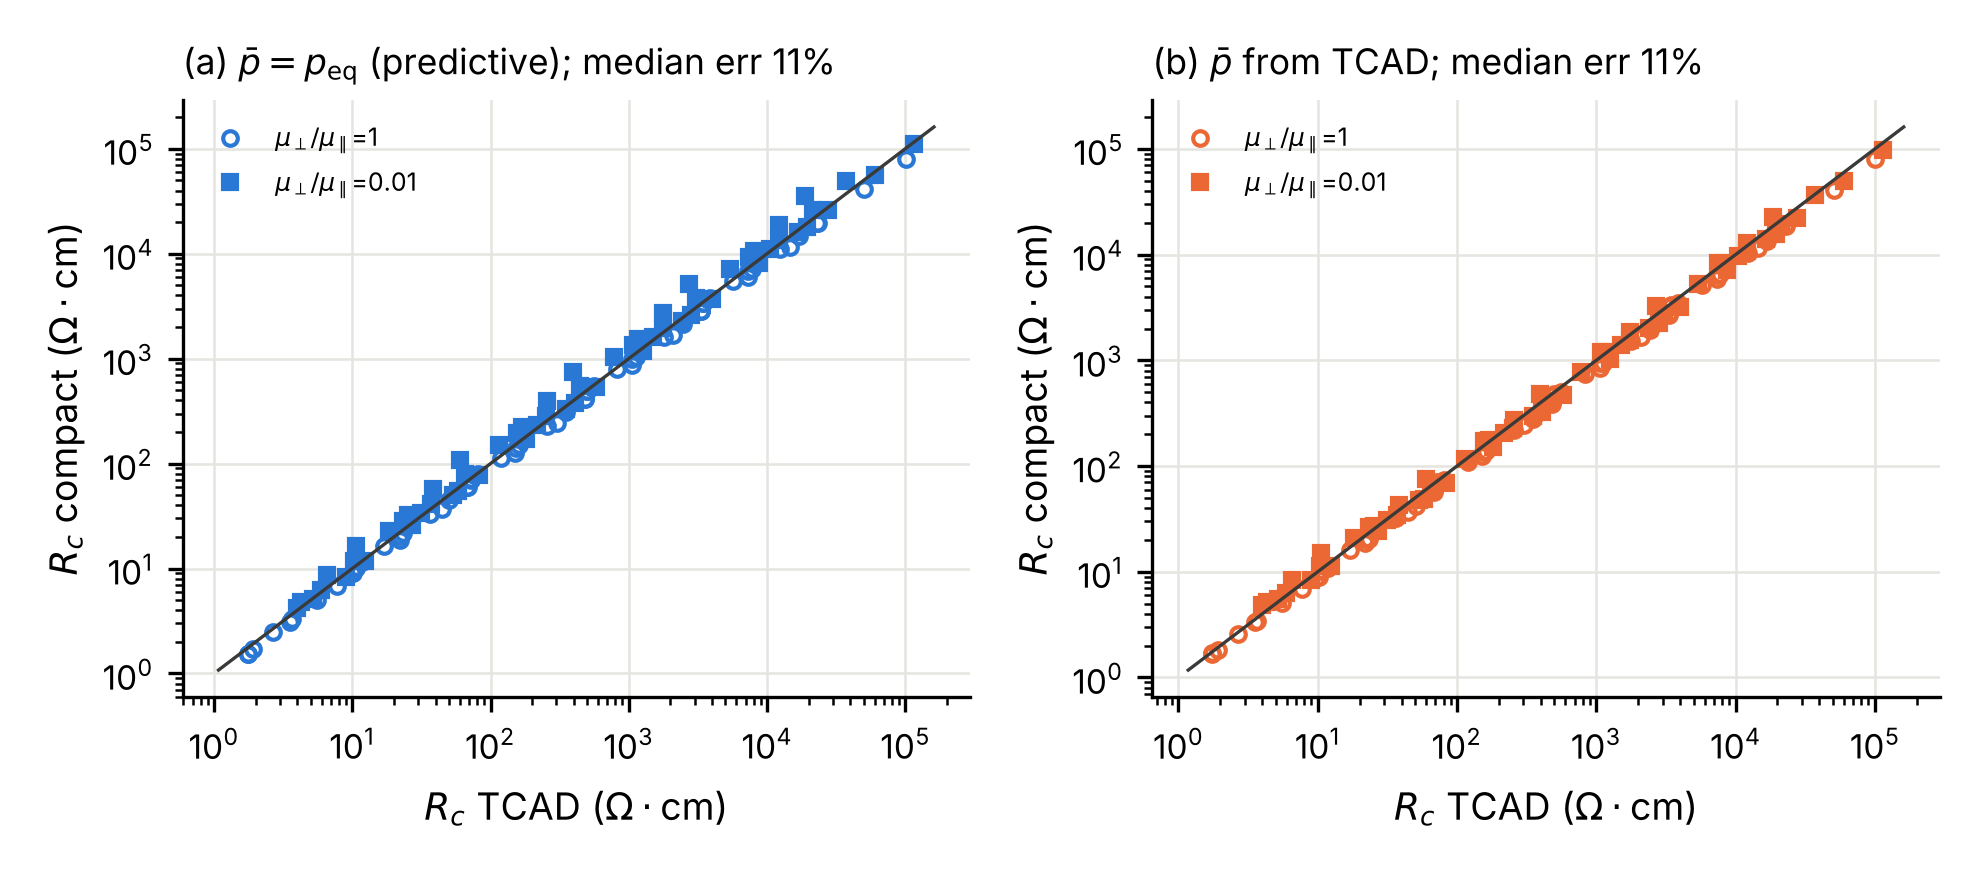
\includegraphics[width=0.96\textwidth]{fig9_compact_model.png}
\caption{Compact transmission-line model against simulated top-contact $R_c$ (no tunnelling), with (a) $\bar p=p_{\rm eq}$ and (b) $\bar p$ from the simulation.}
\label{fig:compact}
\end{figure}

\subsection{Uncertainty quantification}
\label{sec:uq}
We propagated the uncertainty of the least-known inputs by Monte Carlo sampling: 120 samples, each simulated for both geometries at 4.8 and 5.0~eV, ungated, at 0.05~V. The sampling ranges were:
\begin{itemize}
\item $\Delta E_V\sim\mathcal N(0,0.1~\mathrm{eV})$ and $S\sim U(0.3,1)$, the same for both contacts;
\item $d_{\rm vdW}\sim U(0.2,0.4)$~nm and $\Phi_{\rm vdW}\sim U(1,3)$~eV;
\item log-uniform $\mu_p$ (20--100~cm$^2$/Vs), $\mu_\perp/\mu_\parallel$ (0.002--0.1) and $N_A$ ($10^{15}$--$10^{17}$~cm$^{-3}$);
\item $\varepsilon_r\sim U(5,8)$ and $m_h\sim U(0.1,0.3)$.
\end{itemize}
The resulting 5--95\% range of $R_{\rm tot}$ spans seven to eight orders of magnitude: 61--$1.2\times10^9$~\ohmcm\ for the edge contact at 4.8~eV (Fig.~\ref{fig:uq}a). The band alignment ($\Delta E_V$, Spearman $\rho=-0.63$ to $-0.77$) and the pinning factor ($\rho=-0.69$ to $-0.81$) account for nearly all of the variance. Their first-order indices are 0.47--0.77, while all other parameters stay at or near the estimator's noise floor of about 0.06--0.17 for $n=120$ (Fig.~\ref{fig:uq}b). The \emph{ranking} of the geometries is robust: when both contacts share the same pinning, the edge contact has lower resistance in every sample. The edge/top ratio has a median of 0.24, with a 5--95\% range of 0.07--0.51 at 4.8~eV and 0.08--0.72 at 5.0~eV. The sampled gap parameters correspond to $\mathcal{T}_{\rm vdW}=8\times10^{-4}$--0.13. This excludes the transparent gap that the Au/MoS$_2$ calibration permits; for $\mathcal{T}_{\rm vdW}=1$ the ungated ratio at 4.8~eV would be 0.6--0.9 (Sec.~\ref{sec:vdw}). These variance indices describe $\log_{10}R_{\rm tot}$, which is dominated by the band alignment and pinning. They say little about the top/edge ratio, which depends strongly on $\mathcal{T}_{\rm vdW}$, and the Monte Carlo analysis covers only the ungated state. Absolute resistances, by contrast, cannot be predicted to better than several orders of magnitude until the barrier height of InSe contacts is measured. This is the most valuable single measurement for this system.


\begin{figure}[!htbp]
\centering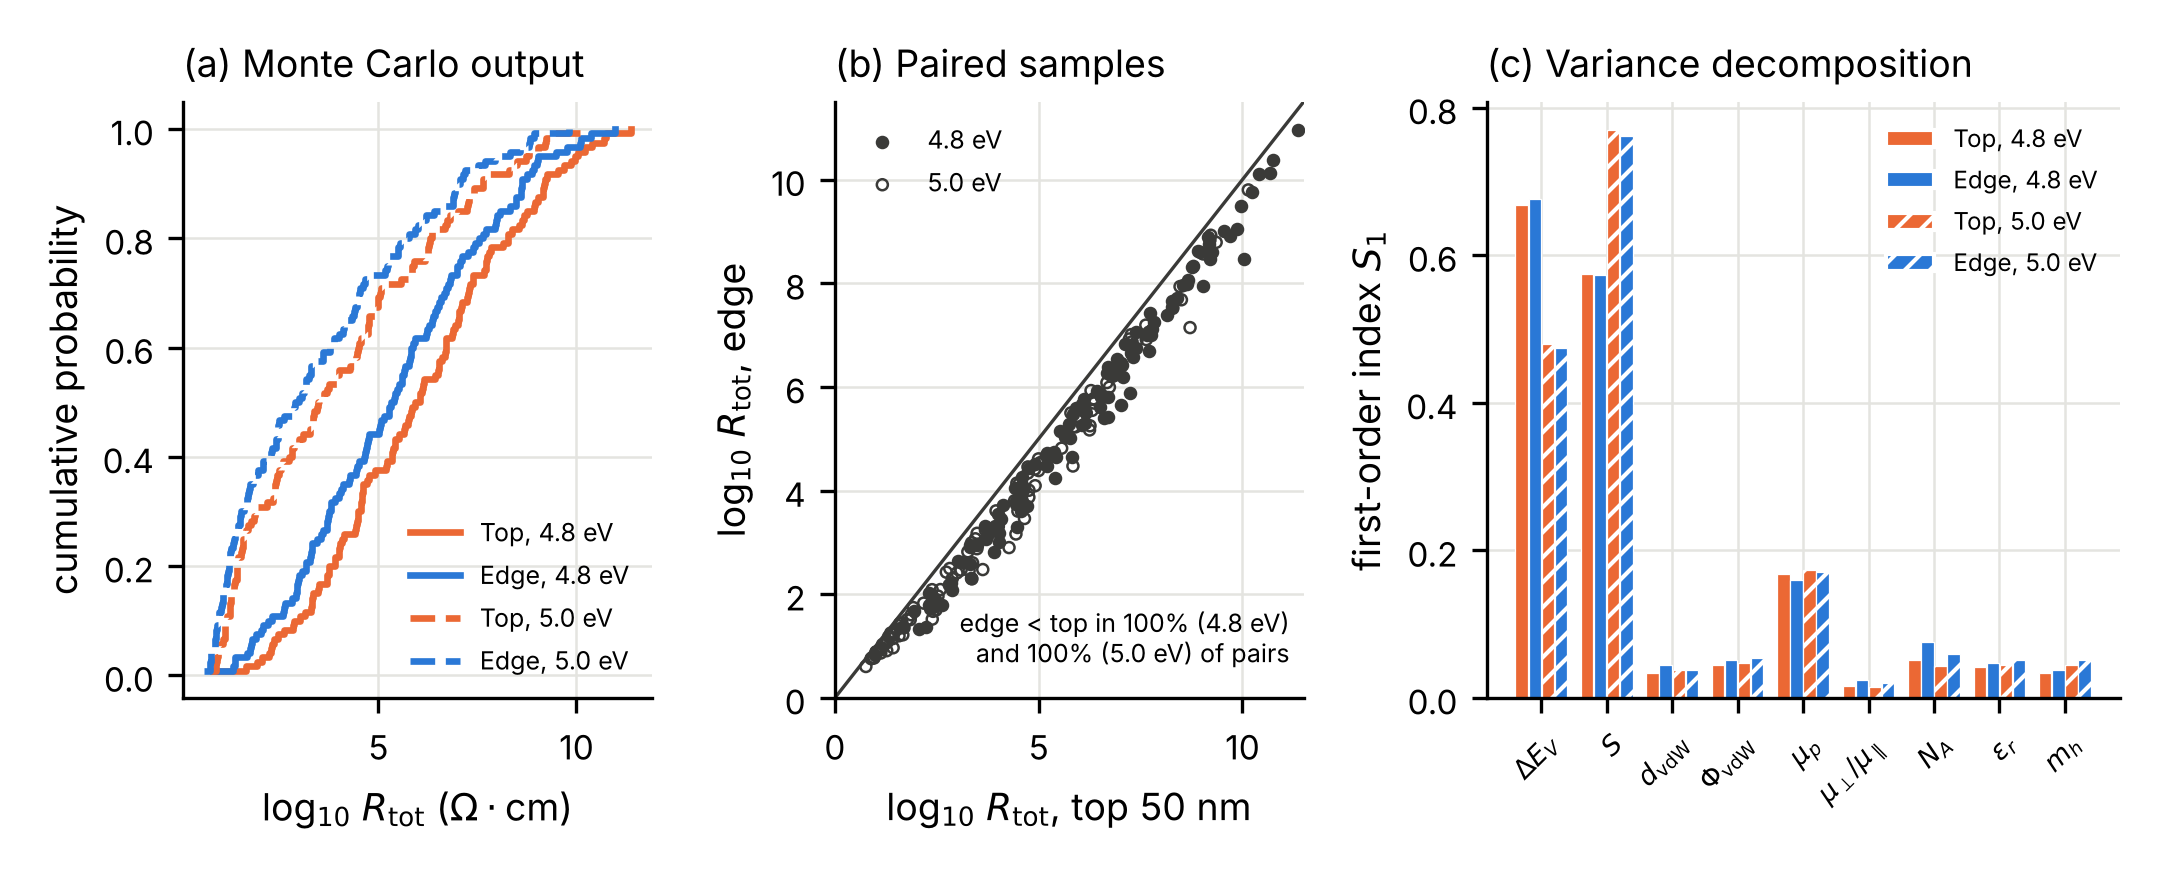
\includegraphics[width=0.96\textwidth]{fig10_uncertainty.png}
\caption{Monte Carlo propagation of parameter uncertainty (ungated, 0.05~V). (a) Cumulative distributions of $\log_{10}R_{\rm tot}$. (b) Paired samples: the same parameter draw simulated for the top (50~nm) and edge contact; points below the diagonal have lower edge resistance. (c) First-order variance indices (colour: geometry; hatching: 5.0~eV). Indices below about 0.06--0.17 are within the noise floor of the estimator for $n=120$ (permutation test).}
\label{fig:uq}
\end{figure}
\begin{figure}[!htbp]
\centering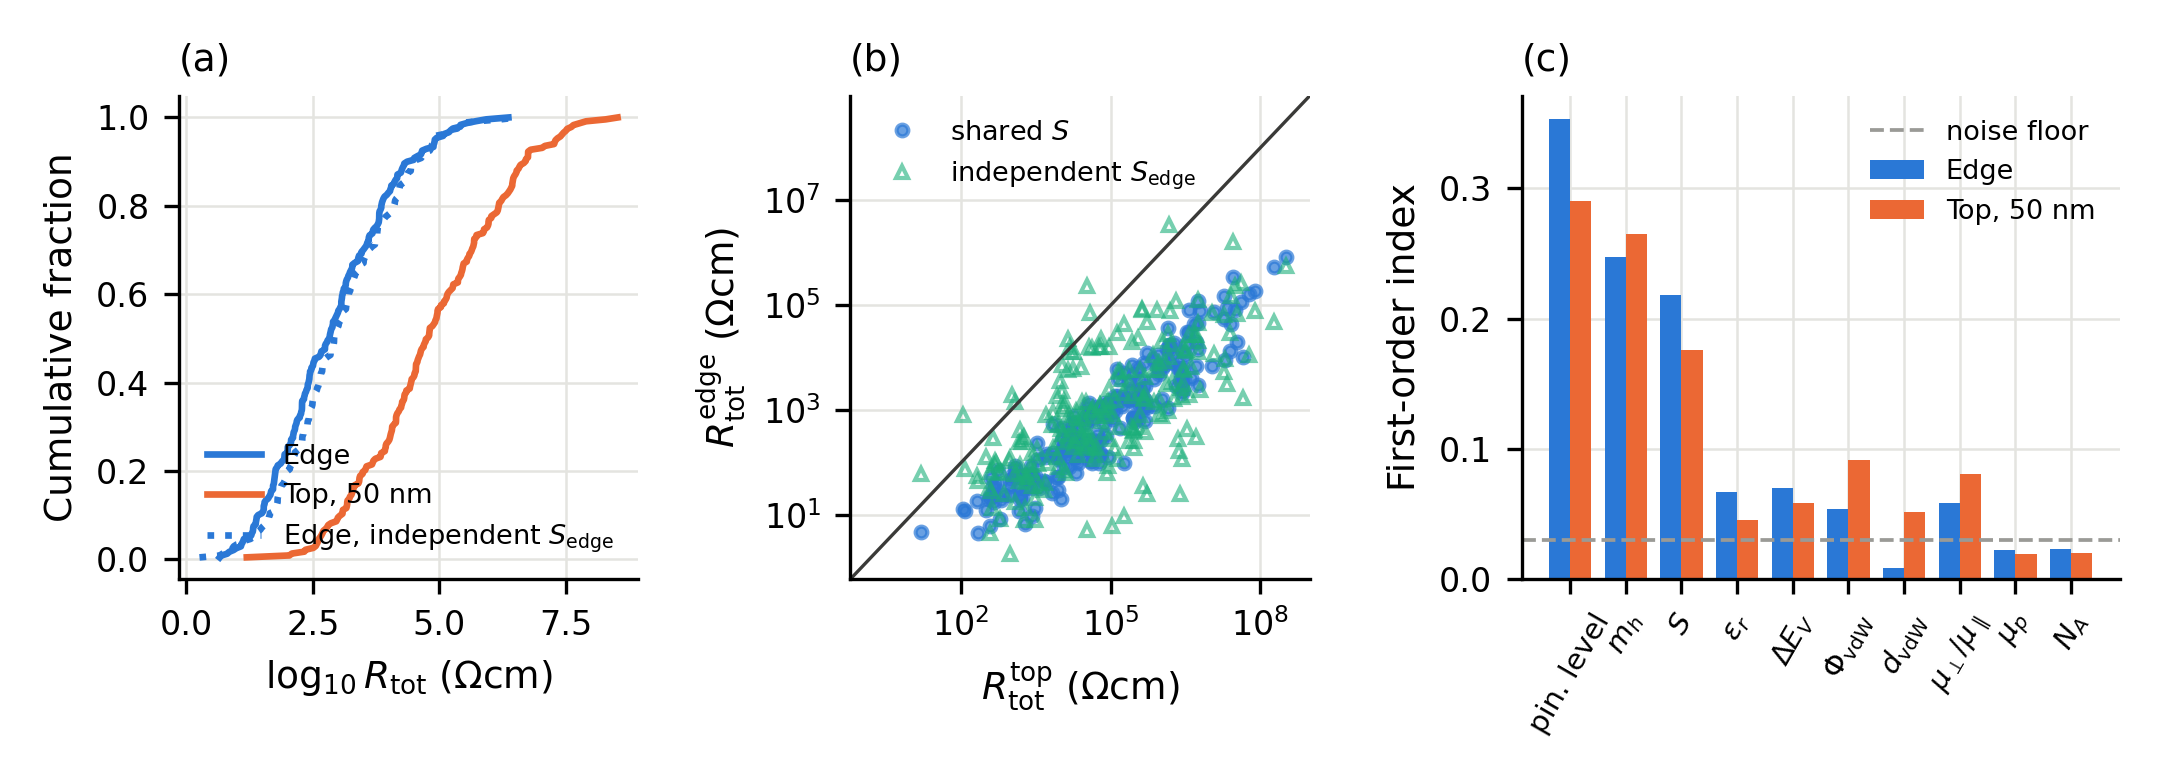
\includegraphics[width=0.96\textwidth]{fig13_uq_gated.png}
\caption{Monte Carlo analysis of the gated on state at the literature alignment (Pt, $V_G=-3$~V, $V_D=0.05$~V, 240 samples). (a) Cumulative distributions of $\log_{10}R_{\rm tot}$. (b) Paired samples with shared $S$ and with independently sampled $S_{\rm edge}$; points below the diagonal have lower edge resistance. (c) Binned first-order indices with the permutation noise floor.}
\label{fig:uqgated}
\end{figure}

\section{Conclusions}
For hole injection into few-layer InSe p-FETs the model gives five design rules:
\begin{enumerate}
\item With the measured pinning of direct metal/InSe contacts ($S=0.05$), every common metal gives a hole barrier of about 1.1~eV and an electron-injecting contact. Hole operation then relies entirely on gate-induced tunnelling, and the metal work function barely matters (2.4$\times$ from Ti to Pt).
\item The barrier must first be lowered by depinning: the measured oxide interlayer brings Pt to 0.52~eV and lowers the contact-limited on-state resistance by up to 700$\times$. A channel-limited device shows a smaller gain, as in the measurements of Ref.~\cite{refchen} (Sec.~\ref{sec:measured}).
\item For hole barriers up to 1~eV, edge contacts beat 50-nm top contacts in the on state, by 14$\times$ at 0.2~eV and 150$\times$ at 1~eV, because they avoid the vdW gap and the slow out-of-plane path. In ungated, barrier-limited operation this holds only if edge contacts are not more strongly pinned than top contacts; in the gated on state it held in 96\% of samples with independently varied pinning. The pinning of edge contacts remains the interface property most worth measuring.
\item Nonlocal tunnelling is essential: thermionic and local enhancement models underestimate the on-current by orders of magnitude.
\item Top contacts have an optimum film thickness of four to six layers. Edge-contacted devices carry more current and need heat removal once the contacts are depinned.
\end{enumerate}
The model is verified, benchmarked on Au/MoS$_2$ with one fitted parameter, anchored to the measured pinning of InSe contacts, and accompanied by a compact model and uncertainty bounds. Its main remaining limitations are the uncertain absolute band alignment of few-layer InSe and the unmeasured pinning of edge contacts. The vdW-gap transmission, the tunnelling mass and the interface thermal resistance are assumed, not measured. The one-dimensional WKB treatment is checked against quadrature on the same band profile (V6) but not against a two-dimensional quantum calculation. The comparison with the InSe measurements of Ref.~\cite{refchen} reproduces the pinning factors, which are inputs, and, for an assumed mobility of 100--200~cm$^2$/Vs, the on-current gain of the oxide interlayer (4--6$\times$ against 3--6$\times$) and both on-currents to within a factor of about two. The mobility and channel length of that experiment are not reported and the on-current is channel-limited, so no InSe contact serves as a calibrated benchmark of the contact resistance. In the gated on state the hole tunnelling mass is, after the pinning level, the largest uncertainty, and on-state resistances at the measured pinning carry a mesh uncertainty of about 15\%.

\section*{Statements and Declarations}
\paragraph{Author contributions} H.A.\ designed the study, developed the code, performed the simulations and analysis, and wrote the manuscript.
\paragraph{Funding} None. \paragraph{Competing interests} None.
\paragraph{Code and data availability} \url{https://github.com/Brukrish2006/InSe-Top-Edge-Contact-Resistace} (\texttt{src\_v3}, \texttt{data\_v3}, \texttt{figures\_v3}). The numbers quoted in Secs.~\ref{sec:measured} and~\ref{sec:heat} are regenerated from \texttt{data\_v3} by \texttt{src\_v3/check\_numbers.py}. The gated Monte Carlo, measured-alignment thermal and thickness runs, mesh study, electron-injection check and comparison with Ref.~\cite{refchen} are produced by \texttt{src\_v3/run\_revision.py} and summarised by \texttt{src\_v3/analyze\_revision.py}. The version of the code and data used for this paper is the repository release tagged \texttt{v3-submission}.

\begin{thebibliography}{99}
\bibitem{refband} D.A.~Bandurin \textit{et al.}, Nat.\ Nanotechnol.\ \textbf{12}, 223 (2017), \doi{10.1038/nnano.2016.242}.
\bibitem{refjiang} J.~Jiang, L.~Xu, C.~Qiu and L.-M.~Peng, Nature \textbf{616}, 470 (2023), \doi{10.1038/s41586-023-05819-w}.
\bibitem{refqin} B.~Qin \textit{et al.}, Science \textbf{389}, 299 (2025), \doi{10.1126/science.adu3803}.
\bibitem{refsong} S.~Song \textit{et al.}, Nat.\ Rev.\ Electr.\ Eng.\ (2025), \doi{10.1038/s44287-025-00251-w}.
\bibitem{refallain} A.~Allain, J.~Kang, K.~Banerjee and A.~Kis, Nat.\ Mater.\ \textbf{14}, 1195 (2015), \doi{10.1038/nmat4452}.
\bibitem{refkang} J.~Kang, W.~Liu, D.~Sarkar, D.~Jena and K.~Banerjee, Phys.\ Rev.\ X \textbf{4}, 031005 (2014), \doi{10.1103/PhysRevX.4.031005}.
\bibitem{refwang} L.~Wang \textit{et al.}, Science \textbf{342}, 614 (2013), \doi{10.1126/science.1244358}.
\bibitem{refguim} M.H.D.~Guimar\~aes \textit{et al.}, ACS Nano \textbf{10}, 6392 (2016), \doi{10.1021/acsnano.6b02879}.
\bibitem{refsangwan} V.K.~Sangwan \textit{et al.}, \textit{Probing vertical conduction in InSe vertical field-effect transistors}, Appl.\ Phys.\ Lett.\ \textbf{115}, 243104 (2019), \doi{10.1063/1.5128808}.
\bibitem{refrai} A.~Rai, V.K.~Sangwan, J.T.~Gish, M.C.~Hersam and D.G.~Cahill, \textit{Anisotropic thermal conductivity of layered indium selenide}, Appl.\ Phys.\ Lett.\ \textbf{118}, 073101 (2021), \doi{10.1063/5.0042091}.
\bibitem{refchen} Y.-H.~Chen \textit{et al.}, \textit{Oxidized-monolayer tunneling barrier for strong Fermi-level depinning in layered InSe transistors}, npj 2D Mater.\ Appl.\ \textbf{3}, 49 (2019), \doi{10.1038/s41699-019-0133-3}.
\bibitem{refguo} Y.~Guo and J.~Robertson, \textit{Band structure, band offsets, substitutional doping, and Schottky barriers of bulk and monolayer InSe}, Phys.\ Rev.\ Mater.\ \textbf{1}, 044004 (2017), \doi{10.1103/PhysRevMaterials.1.044004}.
\bibitem{refszabo} \'A.~Szab\'o, A.~Jain, M.~Parzefall, L.~Novotny and M.~Luisier, \textit{Electron transport through metal/MoS$_2$ interfaces: edge- or area-dependent process?}, Nano Lett.\ \textbf{19}, 3641 (2019), \doi{10.1021/acs.nanolett.9b00678}.
\bibitem{refparto} K.~Parto, A.~Pal, T.~Chavan, K.~Agashiwala, C.-H.~Yeh, W.~Cao and K.~Banerjee, \textit{One-dimensional edge contacts to two-dimensional transition-metal dichalcogenides: uncovering the role of Schottky-barrier anisotropy in charge transport across MoS$_2$/metal interfaces}, Phys.\ Rev.\ Appl.\ \textbf{15}, 064068 (2021), \doi{10.1103/PhysRevApplied.15.064068}.
\bibitem{refarutchelvan} G.~Arutchelvan \textit{et al.}, \textit{From the metal to the channel: a study of carrier injection through the metal/2D MoS$_2$ interface}, Nanoscale \textbf{9}, 10869 (2017), \doi{10.1039/C7NR02487H}.
\bibitem{refmudd} G.W.~Mudd \textit{et al.}, Sci.\ Rep.\ \textbf{6}, 39619 (2016), \doi{10.1038/srep39619}.
\bibitem{refmudd2013} G.W.~Mudd \textit{et al.}, \textit{Tuning the bandgap of exfoliated InSe nanosheets by quantum confinement}, Adv.\ Mater.\ \textbf{25}, 5714 (2013).
\bibitem{refmag} S.~Magorrian, V.~Z\'olyomi and V.~Fal'ko, Phys.\ Rev.\ B \textbf{94}, 245431 (2016), \doi{10.1103/PhysRevB.94.245431}.
\bibitem{refbednarczyk} D.~Bednarczyk and J.~Bednarczyk, \textit{The approximation of the Fermi--Dirac integral $F_{1/2}(\eta)$}, Phys.\ Lett.\ A \textbf{64}, 409 (1978).
\bibitem{refcrowell} C.R.~Crowell and S.M.~Sze, Solid-State Electron.\ \textbf{9}, 1035 (1966).
\bibitem{refieong} M.~Ieong, P.M.~Solomon, S.E.~Laux, H.-S.P.~Wong and D.~Chidambarrao, IEDM Tech.\ Dig., 733 (1998).
\bibitem{refpad} F.A.~Padovani and R.~Stratton, Solid-State Electron.\ \textbf{9}, 695 (1966), \doi{10.1016/0038-1101(66)90097-9}.
\bibitem{refwachutka} G.K.~Wachutka, IEEE Trans.\ Comput.-Aided Des.\ \textbf{9}, 1141 (1990), \doi{10.1109/43.62751}.
\bibitem{refmott} N.F.~Mott and R.W.~Gurney, \textit{Electronic Processes in Ionic Crystals}, 2nd ed., Oxford (1940).
\bibitem{refenglish} C.D.~English, G.~Shine, V.E.~Dorgan, K.C.~Saraswat and E.~Pop, \textit{Improved contacts to MoS$_2$ transistors by ultra-high vacuum metal deposition}, Nano Lett.\ \textbf{16}, 3824 (2016), \doi{10.1021/acs.nanolett.6b01309}.
\end{thebibliography}
\end{document}
